%------------------------------------------------------------------------%
\chapter{MOS transistor}
%------------------------------------------------------------------------%
\centering
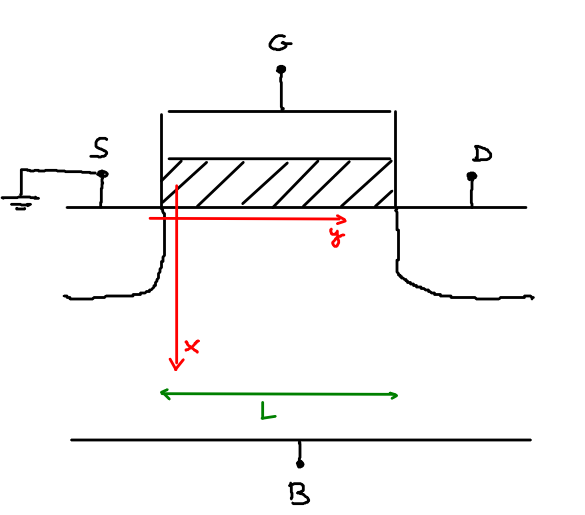
\includegraphics[width=0.35\textwidth]{mos1.png}\\
\raggedright

We start our analysis of the MOS-transistor with the hypotesis of an ideal dialectric ($SiO_2$) and constant doping concentrations.\\
This is an intrinsically bi-dimensional device we will study it in the crossection showed in figure and assuming that all is omogenuos in the ortogonal direction.\\
The most important region of the device is the "channel region" of lenght L that is the one under the gate between the 2 n-doped regions. We will consider in our analysis the two x and y axes placed as in figure.\\
We want to study the electrostatic of this device changing the bias of the four pin; withouth lack of generality since we are intrested in the voltage difference we ground the source for all our analysis.\\


%------------------------------------------------------------------------%
\subsubsection{Working principles}
%------------------------------------------------------------------------%
If $V_{gs}$ is low (until depletion regime) there is no interation between source and drain but if we move to higher $V_{gs}$ (inversion region) we get a lot of electrons from source to drain for the inversion layer so a flow of current it's possible under the gate. The behaviour of the device is like a resistor.\\
Holes have a minor role in the behaviour of the device this is why the MOS transistor, also called field effect unipolar transistor, is an unipolar device.\\

%------------------------------------------------------------------------%
\section{Gradual channel approximation}
%------------------------------------------------------------------------%
To study the electrostatic of this device we have to ideally solve the bi-dimentional Poisson equation but we can simplify our analysis studing only long channel MOS: we define a channel "long" if we can use the gradual channel approximation.\\
The gradual channel approximation says that the electrostatic in the channel region is a quasi 1-D electrostatic and so we can approximate every vertical crossection as a MOS capacitor. If L is large the electric field in the y direction is very small and the dominant electric field is in the vertical direction.\\
We can use the resuslts we have from the MOS capacitor.\\

\centering
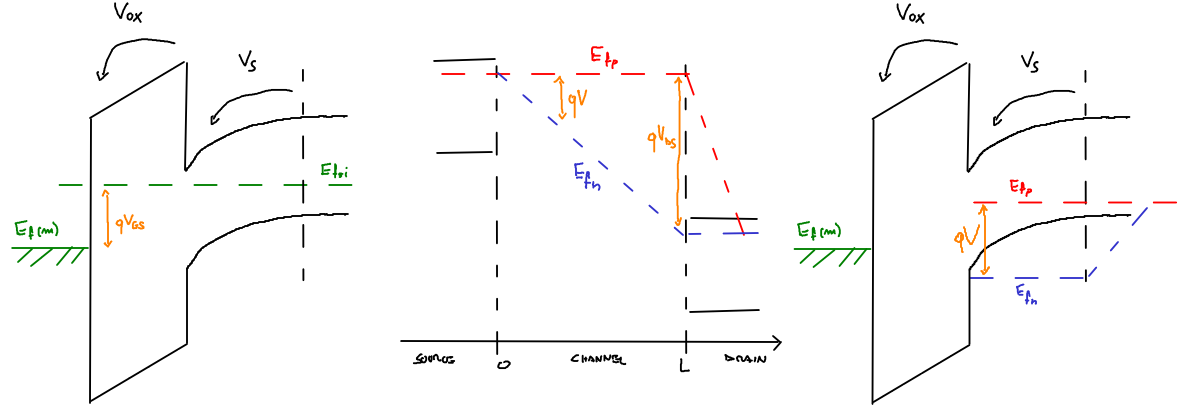
\includegraphics[width=0.9\textwidth]{mos2.png}\\
\raggedright

Assuming $V_{gs}>0$ and $V_{ds}>0$ along the first crossection we get what we've sudied with the MOS capacitor but in the second crossection we have a split of the 2 quasi-Fermi levels due to the shift downwards of the drain bands of an amount of $qV_{ds}$ so the substrate is no longer at th. eq. and so also the frist graph have to be changed. $E_{fp}$ remains constant over the channel but $E_{fn}$ changes.\\
Placing the 0 level to $E_{fp}$ that doesn't change we introduce the parameter 
\begin{equation}
V=-\frac{E_{fn}(y)}{q}=V(y)
\end{equation}
V goes from 0 (at the source) to $V_{ds}$ (at the drain).\\


%------------------------------------------------------------------------%
\section{Poisson equation}
%------------------------------------------------------------------------%
Looking at the last band diagram we plotted the poisson equation it's very similar to the one of an MOS capacitor the only difference is in the n term that now is 
\begin{equation}
n=\frac{n_i^2}{N_a}e^{q\Delta \phi /kT}e^{-qV/kT}
\end{equation}
The last exponential takes into account the decrease of the quasi-Fermi level for electrons that is far from the conduction band wrt the MOS capacitor case.\\

\vspace{5mm}

Check: if $n(0)=\frac{n_i^2}{N_a}e^{qV_s/kT}e^{-qV/kT}$ let's consider $n(0)=N_a$ (stong inversion at the source) we get $e^{-2|\phi_b|/kT}e^{-qV/kT}e^{qV_s/kT}=1$ and so
\begin{equation}
-2|\phi_b|+V_s-V=0 \ \ \ \ V_s=2|\phi_b|+V
\end{equation}

\vspace{5mm}

Repeating all calcualtion done for the expression we get is similar to the one with the mos capacitor
\begin{equation}
\left(\frac{d\Delta\phi}{dx}\right)^2=\frac{2kTN_a}{\varepsilon_{si}}[e^{-q\Delta\phi/kT}+\frac{q\Delta\phi}{kT}-1+\frac{n_i^2}{N_a^2}\left((e^{q\Delta\phi/kT}-1)e^{-qV/kT}-\frac{q\Delta\phi}{kT}\right)]
\end{equation}
we change the term that takes into account the electron concentration.\\
With this result we know $F_x^2=\left(\frac{d\Delta\phi}{dx}\right)^2$ and that $F_x(x,y)=F_x(\Delta\phi,V)$.\\

%------------------------------------------------------------------------%
\section{Charge in the substrate}
At the silicon surface the field is $F_s=F(0,y)=F(V_s,V)$ from this with the Gauss law we can say that the charge in the substrate (in weak and strong inversion that are the intresting regimes) is 
\begin{equation}
Q_s\simeq-\sqrt{2\varepsilon_{si}kTN_a}\left(\frac{qV_s}{kT}+\frac{n_i^2}{N_a^2}e^{q(V_s-V)/kT}\right)^{1/2}
\end{equation}
Now to divide the contribution coming from the inversion charge and from the depletion layer we have to refer to the different regimes.\\

%------------------------------------------------------------------------%
\subsection{Charge in weak inversion}
In weak inversion we have that $Q_s=Q_{inv}+Q_{dep}$  using Taylor expansion of the exponential term we arrive at the following results
\begin{equation}
Q_{dep}=-\sqrt{2\varepsilon_{si}qN_aV_s}\ \ \ \ \ \ \ \ \ \   Q_{inv}=-\sqrt{\frac{\varepsilon_{si}qN_a}{2V_s}}\frac{kT}{q}\frac{n_i^2}{N_a^2}e^{q(V_s-V)/kT}
\end{equation}
In the y axes $E_c, E_v$ are flat and $F_y^{weak.i}\simeq0$ so current transport is a diffusion process and the flow of holes is negligible.

%------------------------------------------------------------------------%
\subsection{Charge in strong inversion}
The expression seen before for the depletion charge is no longer valid in strong inversion becuse the concentration of electrons isn't negligible and the inversion layer charge chanege the F profile \\


\centering
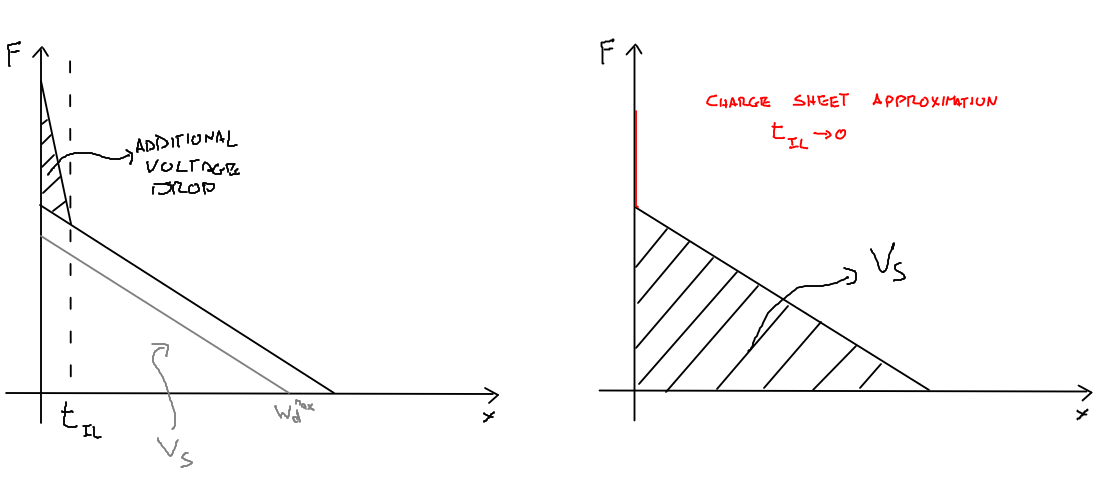
\includegraphics[width=0.7\textwidth]{csa.png}\\
\raggedright

To recover that expression we can make a charge sheet approximation that is considering the thikness of the inversion layer so small to be negligible to have a graph like in figure above.\\
Making this approximation we conclude that
\begin{equation}
Q_{dep}=-\sqrt{2\varepsilon_{si}qN_aV_s} \ \ \ \ \ \ \ \ Q_{inv}=Q_s-\sqrt{2\varepsilon_{si}qN_aV_s}
\end{equation}
In stong inversion the electrons concentration is no more negligible and at the drain $E_{fn}<E_{fp}$ and bands move downwards form source to drain as the quasi-Fermi level for electrons so there will be a drift flow of electrons and a relevan electric fiels in the y direction.


\centering
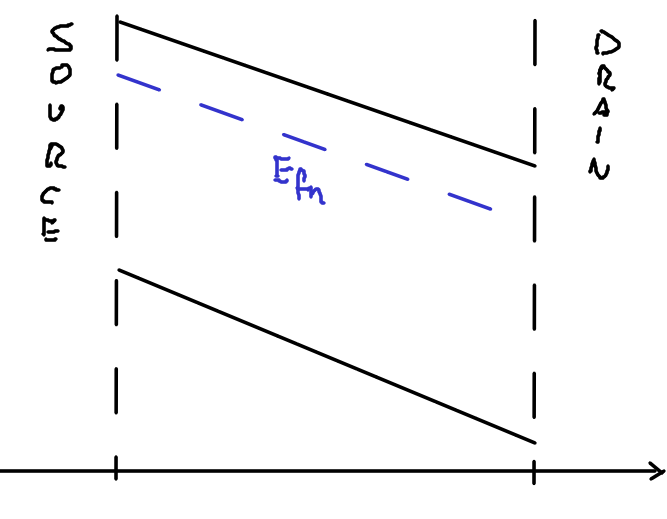
\includegraphics[width=0.35\textwidth]{a1.png}\\
\raggedright


%------------------------------------------------------------------------%
\section{Current behaviour}
%------------------------------------------------------------------------%


\centering
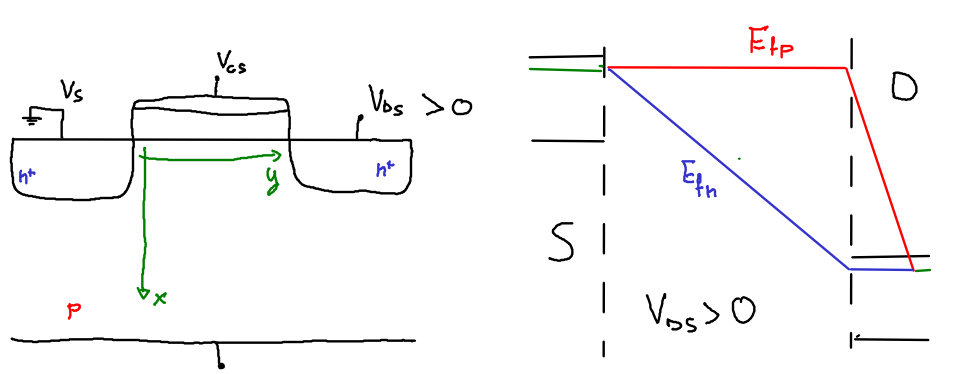
\includegraphics[width=0.5\textwidth]{a2.png}\\
\raggedright


In order to arrive to $V_s(V_{gd},V_{ds})$ we have to use not only $V_{gs}+V_{fb}=V_{s}+V_{ox}=V_{s}-Q_s/C_{ox}$ but also the continuity equation for electrons beacuse the substrate isn't at th.eq.\\
We assume the device stationary and the GR processes negligible so $J_n$ is constant in the channel region. From the interface with the oxide to the substrate the current will decrease due to the decrease of electron concentration but form S-D J will remains constant beacuse the direction is parallel to the current flow so we can say that
\begin{equation}
I_{ds}=-W\int^{t_{inv}}_0 J_n(x)dx
\end{equation}
where $t_{inv}$ is the thikness of the inversion layer and we simply multiply by W beacuse we supposed that everything is constant in that direction. The minus sign is becuse we want positive the current that enter in the drain.\\
So taking into account drift and diffusion process we have 
\begin{equation}
I_{ds}=W\int^{t_{inv}}_0 n\mu_n \frac{dE_{fn}}{dx} dx
\end{equation}
we know that $\frac{dE_{fn}}{dx}=-q \frac{dV}{dy}$ so solving the integral we get
\begin{equation}
I_{ds}=-\mu_nW \frac{dV}{dy}Q_{inv}
\end{equation}
This is the differential form of the drain current in MOS transistor and making another step of integration we come to 
\begin{equation}
I_{ds}=-\mu_n\frac{W}{L}\int^{V_{ds}}_0Q_{inv}dV
\end{equation}
the integral form for drain current. This expressions (differential and interal) are general.\\
\vspace{5mm}

Let's now foucs on storng inversion regime.\\
In this regime we've seen that using the charge sheet approximation $Q_{inv}=Q_s+\sqrt{2\varepsilon_{si}qN_aV_s}$ if we combine this equation with 
\begin{equation}
Q_s=-\sqrt{2\varepsilon_{si}kTN_a}\left(\frac{qV_s}{kT}+\frac{n_i^2}{N_a^2}e^{q(V_s-V)/kT}\right)^{1/2}
\end{equation}
 and with $V_{gs}+V_{fb}=V_{s}-Q_s/C_{ox}$ we get that $V_s\simeq2|\phi_b|+V$ and $Q_s=-C_{ox}(V_{gs}-V_{fb}-V_{s})$ if we use this two equation with the first one (inversion charge) we get that
\begin{equation}
Q_{inv}\simeq -C_{ox}(V_{gs}-V_{fb}-2|\phi_b|-V)+\sqrt{2\varepsilon_{si}qN_a(2|\phi_b|+V)}
\end{equation}
we will not solve this equation but we will consider some different regimes


%------------------------------------------------------------------------%
\subsection{Ohmic regime $V_{ds}<<2|\phi_b|$}

If $V_{ds}$ is small also V will be small so we can neglect that contribution 
\begin{equation}
Q_{inv}\simeq -C_{ox}(V_{gs}-V_{fb}-2|\phi_b|-\frac{Q_{dep}^{max}}{C_{ox}})\simeq -C_{ox}(V_{gs}-V_t)
\end{equation}
so putting this result in the integral form for the current and solving the integral we get
\begin{equation}
I_{ds}=\mu_nC_{ox}\frac{W}{L}(V_{gs}-V_t)V_{ds}
\end{equation}
This is the expression for ohmic regime the current is proportional to $V_{ds}$.\\
\begin{wrapfigure}{i}{0pt}
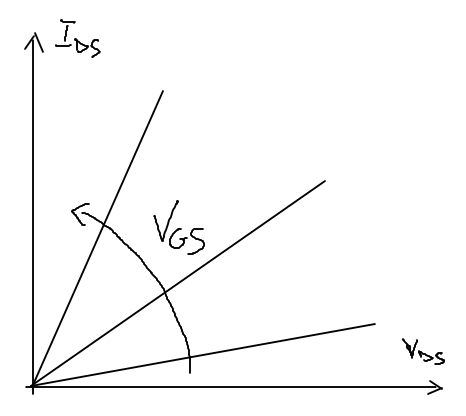
\includegraphics[width=0.17\textwidth]{ohmreg.png}
\end{wrapfigure}

The inversion charge does not change from source to drain and beacuse $V_{ds}$ is very small the electrostatic is almost uniform along the channel.\\

It's like having a resistor in the channel that can be modulate by $V_{gs}$. We can define a resistivity for the channel as 
\begin{equation}
R_{ch}=(\frac{\partial I_{ds}}{\partial V_{ds}})^{-1}=\frac{1}{\mu_nC_{ox}(V_{gs}-V_{t})}\frac{L}{W}=\rho_{sh}^{ch}\frac{L}{W}
\end{equation}
We espect the field constatn and so equal to $V_{ds}/L$.\\

\subsection{Parabolic regime $V_{ds}<2|\phi_b|$}
Now $V_{ds}$ is no more negliglibe but enought small to make a Taylor expansion of the second terms as
\begin{equation}
Q_{inv}\simeq -C_{ox}(V_{gs}-V_{fb}-2|\phi_b|-V)+\sqrt{2\varepsilon_{si}qN_a2|\phi_b|}(1+\frac{1}{2}\frac{V}{2|\phi_b|})=-[...]+\sqrt{\frac{\varepsilon_{si}qN_a}{4|\phi_b|}}V=-[...]+|Q_{dep}^{max}|+C_{dep}V
\end{equation}
and so re-writing the equation
\begin{equation}
Q_{inv}\simeq-C_{ox}(V_{gs}-V_{fb}-2|\phi_b|-\frac{Q_{dep}^{max}}{C_{ox}}-V(1+\frac{C_{dep}}{C_{ox}}))=-C_{ox}(V_{gs}-V_t-mV)
\end{equation}
The term -mV is an increase of the threshold voltage from source to drain.\\
The inversion charge is decreasing from source to drain; putting this equation in the integral we get 
\begin{equation}
I_{ds}=\mu_nC_{ox}\frac{W}{L}[(V_{gs}-V_t)V_{ds}-\frac{mV_{ds}^2}{2}]
\end{equation}
we have a parabolic behaviour of the current. If $V_{ds}$ is small we can neglect the quadratic term and so recovering the previous condition.


\centering
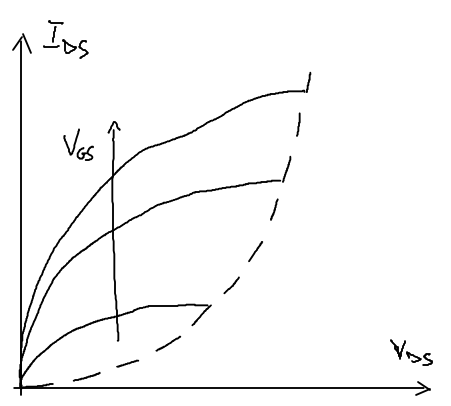
\includegraphics[width=0.25\textwidth]{parabreg.png}\\
\raggedright



\subsection{Saturation point}
We can call the current and voltage of the vertex of the parabola saturation's one 
\begin{equation}
V_{ds}^{sat}=\frac{V_{gs}-V_t}{m}\ \ \ \ \ \ \ \ I_{ds}^{sat}=\mu_nC_{ox}\frac{W}{L}\frac{(V_{gs}-V_t)^2}{m}=\mu_nC_{ox}\frac{W}{L}\frac{(V_{ds}^{sat})^2}{m}
\end{equation}
Increasing $V_{ds}$ we increase the electric field and decrease the charge (so we get a more resistive channel). At $V_{ds}^{sat}$ the charge at the drain is 
\begin{equation}
Q_{inv}(y=L)=-C_{ox}(V_{gs}-V_t-m \frac{V_{gs}-V_t}{m})=0
\end{equation}
this is called the pinch off conditon of the transistor. If from the saturation point on we keep using the previous equation we get a reduction of the current that has no sense.\\

\subsubsection{Mathematical explanation of dicendent parabola}

\centering
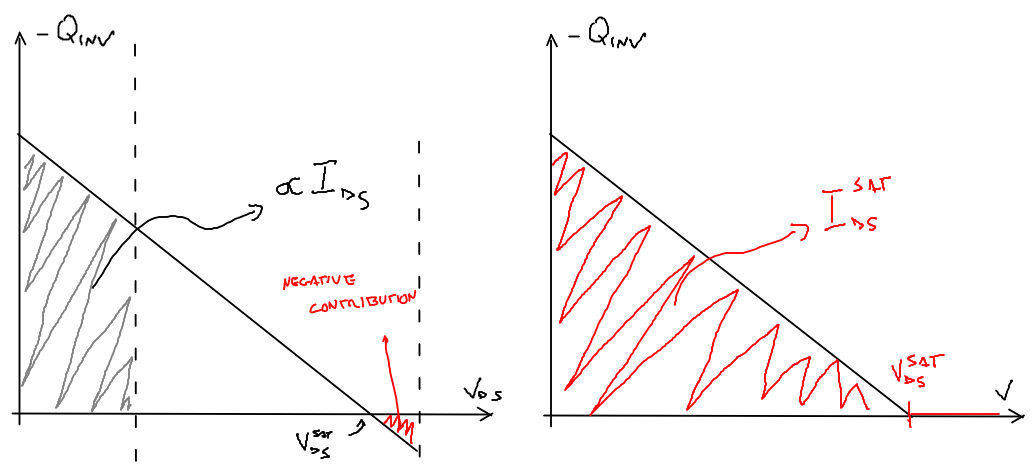
\includegraphics[width=0.7\textwidth]{mathexpl.png}\\
\raggedright

Let's consider $-Q_{inv}(V_{ds})$ we calculated the area of this expression to find the current so the area under the rect in the graph is proportional to the current. When $V_{ds}=V_{ds}^{sat}$ we are at the vertex of the parabola and so the current is proportional to the area of the triangle.\\
From there on we add negative area contribution that has no sense it's like accumuling holes in the inversion layer. At the drain we were at the limit of strong inversion regime if we increase $V_{ds}$ over the saturation point we enter at the drain at weak inversion regime where electrons concentration can be apporoximated as negligible. The real graph of the inversion charge becomes zero over the saturation voltage so from the vertex on the current remains constant.\\

%------------------------------------------------------------------------%
\subsubsection{Physical explanation of dicendent parabola}


\centering
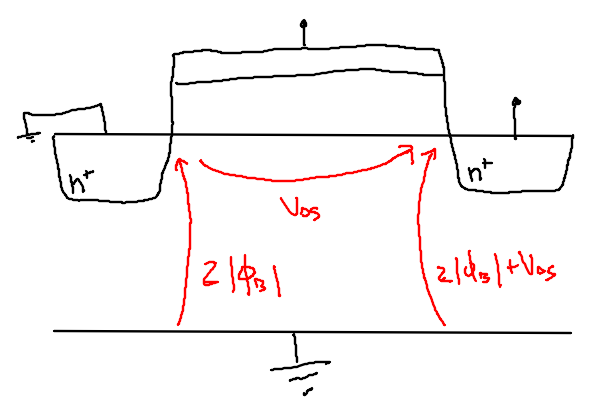
\includegraphics[width=0.35\textwidth]{f1.png}\\
\raggedright

Start from the condition of $V_{gs}$ big enough to have strong inversion in the channel; at source we will have a single Fermi level at drain 2 Fermi levels displaced by $qV_{ds}$. Since we are keeping strong inversion the bands must move down to keep $E_{fn}$ close to $E_c$.\\

\centering
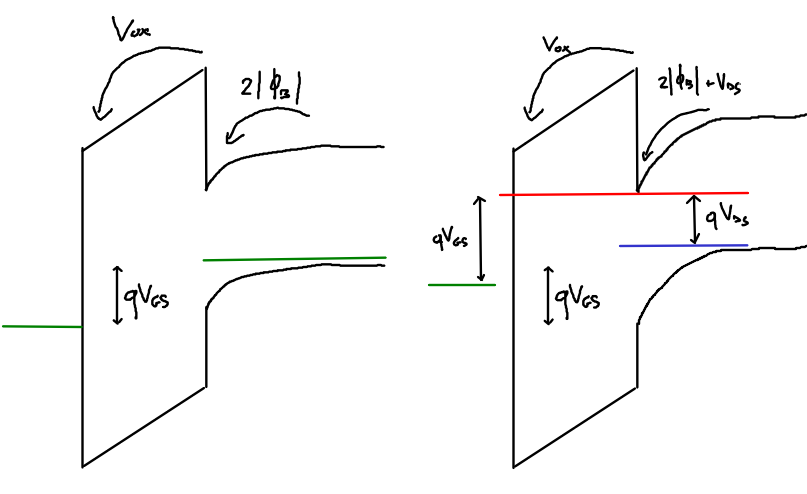
\includegraphics[width=0.7\textwidth]{f2.png}\\
\raggedright


Let's look at $V_s(y=L)$ at the drain side as $V_{ds}$ increases; if $V_{ds}$ is small $V_s\simeq 2|\phi_b|$ and increasing the drain voltage we will increase also $V_s\simeq 2|\phi_b|+V_{ds}$. When $V_{ds}^{sat}$ is reached what happen.\\


\centering
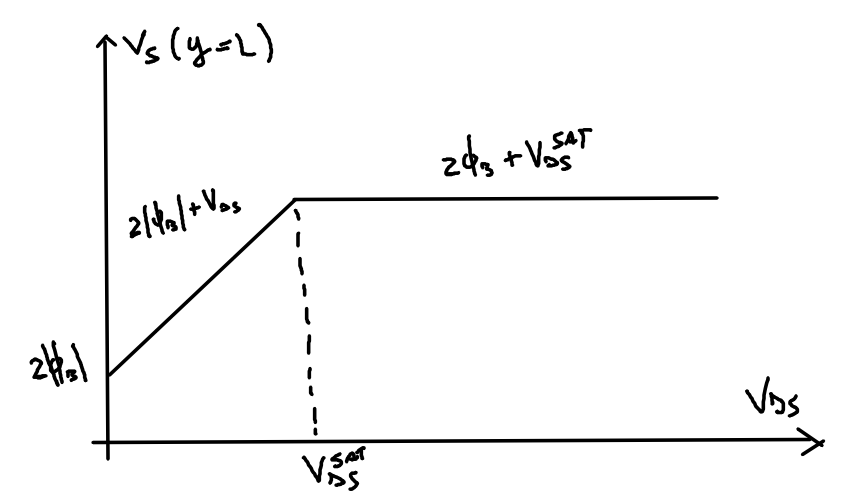
\includegraphics[width=0.35\textwidth]{f3.png}\\
\raggedright


We consider the $V_s-V_{ds}$ plot at constant $V_{gs}$ by increasing $V_{ds}$ we have $V_s$ closer to the $V_t'$ (threshold voltage also at the drain) and the onset of weak inversion. When we reach the intersection $V_s$ does not change any longer and the drain loses control of the electrostatics; the channel and the elctric fields in the y direction does not change anymore so we reach the maximum band banding.\\ $Q_{inv}=0$ does not means really zero but negligible electron concentration (we are in weak inversion).\\
The parameter $m=1+\frac{C_{dep}}{C_{ox}}$ involves doping concentration and oxide thikness and express how much of $V_g$ drops over the substrate; for a good mos m=1,1-1,4.\\



%------------------------------------------------------------------------%
\section{Over the saturation point}
%------------------------------------------------------------------------%

We still don't know $E_{fn}$ along the channel or the voltage drop in function of y.\\
From the differential from of the drain current we have $I_{ds}=-\mu_nW \frac{dV}{dy}Q_{inv}$ we can integrate this expression up to a potential V in a point y
\begin{equation}
\int_0^yI_{ds}dy=\int^V_0-\mu_nWQ_{inv}dV
\end{equation}
\begin{equation}
I_{ds}y=\int^V_0\mu_nWC_{ox}(V_{gs}-V_t-mV)dV=\mu_nWC_{ox}[(V_{gs}-V_{t})V-\frac{mV^2}{2}]
\end{equation}
but we know from the parabolic regime another expression for $I_{ds}=\mu_n \frac{W}{L}C_{ox}[(V_{gs}-V_{t})V_{ds}-\frac{mV_{ds}^2}{2}]$ so we can get V(y) as
\begin{equation}
V(y)=\frac{V_{gs}-V_{t}}{m}-\sqrt{\left(\frac{V_{gs}-V_{t}}{m}\right)^2-\frac{2y}{L}\left(\frac{V_{gs}-V_{t}}{m}\right)V_{ds}+\frac{y}{L}V_{ds}^2}
\end{equation}
from that we know $E_{fn}$ beacuse $V=-E_{fn}/q$.\\
This result is general but we will study it in the various regime; in ohmic region $V_{ds}$ is small so we can neglect the quadratic term and extract the $\frac{V_{gs}-V_{t}}{m}$ term from the sqare root, in this way making a Taylor expansion we get
\begin{equation}
V(y)\simeq\frac{V_{gs}-V_{t}}{m}-\frac{V_{gs}-V_{t}}{m}\sqrt{1-\frac{2y}{L}V_{ds}/\left(\frac{V_{gs}-V_{t}}{m}\right)}\simeq \frac{V_{gs}-V_{t}}{m}-\frac{V_{gs}-V_{t}}{m}\left(1-\frac{y}{L}V_{ds}/\left(\frac{V_{gs}-V_{t}}{m}\right)\right)
\end{equation}
\begin{equation}
V\simeq \frac{V_{ds}}{L}y
\end{equation}
resonable result when the channel is uniform and we said that $\frac{dV}{dy}$ has to be constan so V linear function of y. We get a constant drift contribution over the channel.\\

\begin{wrapfigure}{i}{0pt}
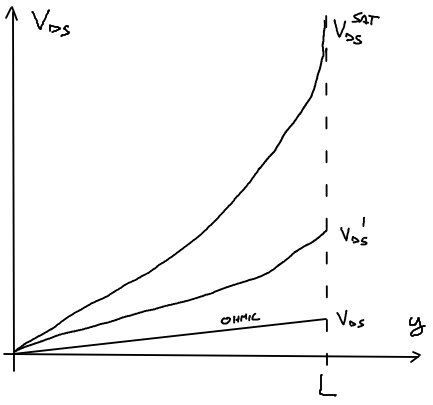
\includegraphics[width=0.2\textwidth]{g1.png}
\end{wrapfigure}


Increasing the drain voltage we enter in the parabolic regime and the charge will decrease and ,beacuse the differential form of the current must be always valid , $\frac{dV}{dy}$ must increase (we need higher electric field). We increase the slope of the rect form source to drain.\\
At pinch off point we have no charge in L so at $V_{ds}^{sat}$ we reach L with vertical tangent. This condition means infinite electric field in y direction so $F_y$ is no more negligible and the gradual channel approximation is no longer valid.\\
We have to study the 2D Poisson equation. We will not study it mathematically but let's see the results.\\

\centering
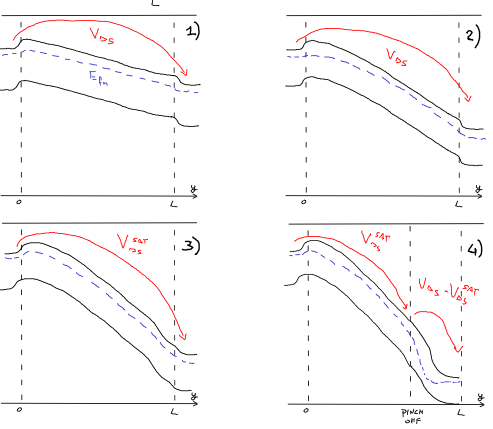
\includegraphics[width=0.6\textwidth]{pograph.png}\\
\raggedright

In ohmic regime $V_{ds}$ is small so we get the 1) graph.\\
Increasing $V_{ds}$ we increase the slope of $E_{fn}$ that change like figure 2).\\
We reach the pinch off point large F very large tangent at L but not infinite like in figure 3).\\
Using gradual channel approximation we sad that the drain over the saturation voltage loses control of the band banding this is unreasonable; in reality the pinch off point moves leftwards for voltages higher than saturation at draid leaving a potential $V_{ds}^{sat}$ from source to pinch-off and form pinch-off to drain $V_{ds}-V_{ds}^{sat}$. like in figure 4).
This effect acts like a reduction of the L of the channel.\\
In the x axis the band diagram is purely 2D band-diagram; the maximum electron concentration is no more at the interface but it's spread in the vertical direction.\\ Beyond the pinch-off we have a depleted region.\\

\centering
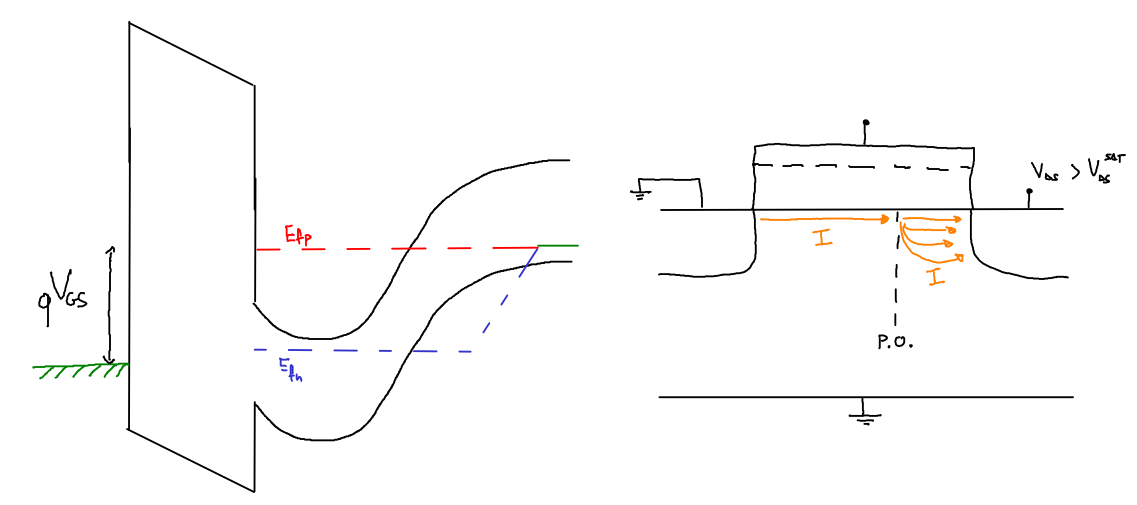
\includegraphics[width=0.6\textwidth]{2delectro.png}\\
\raggedright

%------------------------------------------------------------------------%
\section{Transcaracteristic}
%------------------------------------------------------------------------%

\centering
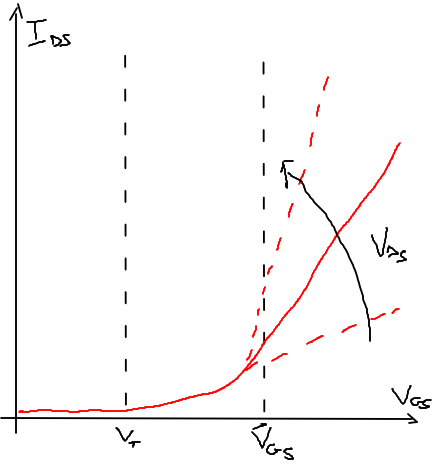
\includegraphics[width=0.35\textwidth]{transcaracteristic.png}\\
\raggedright

We assume $V_{ds}$ set and we change $V_{gs}$ and we want to know the current profile.\\
First region we get $V_{gs}<V_{t}$ so we are in accumulation or weak inversion region so the current is negligible.\\
When we reach $V_{gs}=V_t$ we enter in the on-state regime we are at saturation beacuse we have $V_{t}$ at the source but going to the drain the thrashold voltage increase so we don't have threshold there. $I_{ds}^{sat}=\mu_nC_{ox}\frac{W}{L}\frac{(V_{gs}-V_t)^2}{2m}$ so we have a parabolic dependance.\\
We increase $V_{gs}$ until we reach the threshold condition also at the drain at the voltage $V_t'=V_t+m V_{ds}=\overline{V_{gs}}$  in this case the current is $I_{ds}=\mu_nC_{ox}\frac{W}{L}[(V_{gs}-V_t)V_{ds}-\frac{mV_{ds}^2}{2}]$ so a linear dependance.\\

%------------------------------------------------------------------------%
\section{Small signal parameters}
%------------------------------------------------------------------------%

%------------------------------------------------------------------------%
\subsection{Transonductance $g_m$}
If we slightly move $V_{gs}$ we change the current flow so we can define a small signal transconductance as $g_m=\left(\frac{\partial I_{ds}}{\partial V_{gs}}\right)_{V_{ds}}$ that in ohmic-parabolic and saturation regime is
\begin{equation}
g_m^{ohmic}=\mu_nC_{ox}\frac{W}{L}V_{ds} \ \ \ \ \ \ \ \ \ \ \  g_m^{sat}=\mu_nC_{ox}\frac{W}{L}\frac{V_{gs}-V_t}{m}
\end{equation} 

\centering
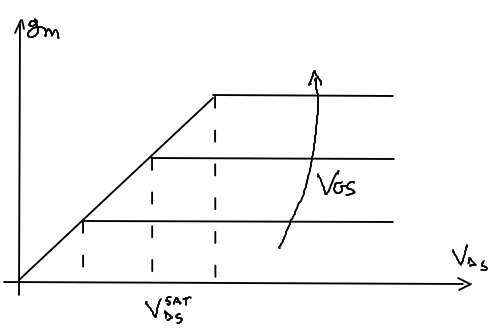
\includegraphics[width=0.35\textwidth]{gmmos.png}\\
\raggedright

%------------------------------------------------------------------------%
\subsection{Transconductrance $g_d$}
We can define also $g_d=\left(\frac{\partial I_{ds}}{\partial V_{ds}}\right)_{V_{gs}}$ that for ohmic and parabolic regime is
\begin{equation}
g_d^{ohmic}=\mu_nC_{ox}\frac{W}{L}[(V_{gs}-V_t)-mV_{ds}] \ \ \ \ \ \ \ \ \ \ g_d^{sat}=0
\end{equation}
This last result is obviously an approximation becuse we implicitedly used the gradual channel approximation that is not valid in saturation regime.\\
Using 2D Poisson equation we get that the pinch-off point moves from drain to source if $V_{ds}>V_{ds}^{sat}$; this phenomena is equivalent to a reduction of the L of the transistor that means an increase of current.\\

\centering
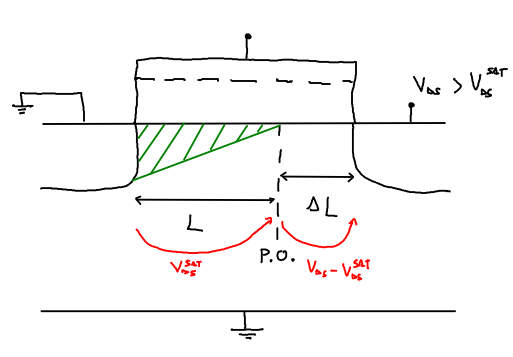
\includegraphics[width=0.35\textwidth]{early.png}\\
\raggedright

For the sake of semplicity we suppose $\Delta L\propto V_{ds}$ with direct proportionality so
\begin{equation}
\Delta L =\frac{V_{ds}-V_{ds}^{sat}}{F_p}
\end{equation}
where $F_p$ is the average field in the $\Delta L$ region. Moving to larger $V_{ds}$ than $V_{ds}^{sat}$ we can write 
\begin{equation}
I_{ds}=I_{ds}^{sat}\frac{L}{L-\Delta L }=I_{ds}^{sat}\frac{1}{1-\frac{\Delta L}{L}} 
\end{equation}
refering to a long channel device $\Delta L$ is very small compared to L so we can make a Taylor expansion obtaining 
\begin{equation}
I_{ds}=I_{ds}^{sat}(1+\frac{\Delta L}{L})=I_{ds}^{sat}(1+\frac{V_{ds}-V_{ds}^{sat}}{LF_p})
\end{equation}
we get a linear increase of the current increasing $V_{ds}$ and also a larger slope ot the rect with higher currents.\\
So the real output resistance is 
\begin{equation}
g_d=\left(\frac{\partial I_{ds}}{\partial V_{ds}}\right)^{-1}_{V_{gs}}=\frac{LF_p}{I_{ds}^{sat}}
\end{equation}
that is a strong function of L.\\

\centering
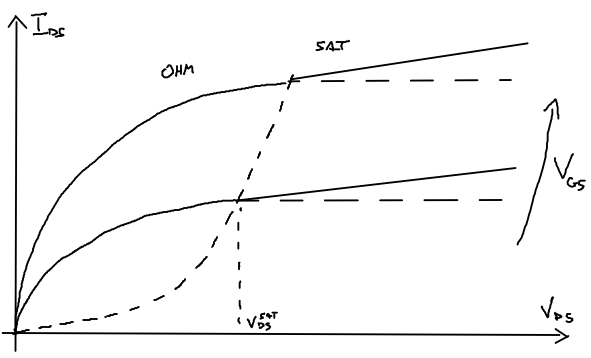
\includegraphics[width=0.45\textwidth]{early1.png}\\
\raggedright

%------------------------------------------------------------------------%
\subsection{Capacitive terms}
In this section we will introduce only intrinsic capacitive terms.\\
We define $Q_c$ total charge in the inversion layer as 
\begin{equation}
Q_c=W\int^L_0Q_{inv}dy=[C]
\end{equation}
if we change the integration variable by multipling and dividing by dV we get
\begin{equation}
Q_c=W\int^{V_{ds}}_0Q_{inv}dV\frac{dy}{dV}
\end{equation}
from the differential form of the drain current we know that $I_{ds}=-\mu_nW \frac{dV}{dy}Q_{inv}$ so using this expression to derive $\frac{dV}{dy}$ we get
\begin{equation}
Q_c=-\mu_n \frac{W^2}{I_{ds}}\int^{V_{ds}}_0 C_{ox}^2(V_{gs}-V_t-mV)^2dV
\end{equation}
solving the integral and unsing the expression for the current we get the final result
\begin{equation}
Q_c=-WLC_{ox}'\frac{2}{3} \frac{m^2V_{ds}^2 + 3(V_{gs}-V_t)^2 -3mV_{ds}(V_{gs}-V_t)}{2(V_{gs}-V_t)-mV_{ds}}
\end{equation}
This formula is general and valid for all on-state regimes but we can apporximate it for the ohmic regime when $V_{ds}\simeq 0$ and for the saturation regime where $V_{ds}^{sat}=(V_{gs}-V_t)/m$ obtaining
\begin{equation}
Q_c=-WLC_{ox}(V_{gs}-V_t)   \ \ \ \ \ \ \ \ \ \ \ [ohmic]
\end{equation}
\begin{equation}
Q_c=\frac{2}{3}  Q_c^{omhic} \ \ \ \ \ \ \ \ \ \ \ [saturation]
\end{equation}
With this two expressions we can derive the gate and the drain capacitance as
\begin{equation}
C_g=-\frac{\partial Q_c}{\partial V_{gs}}|_{V_{ds}}=WLC_{ox}[1-\frac{m^2V_{ds}^2}{3(2(V_{gs}-V_t)-mV_{ds})^2}]
\end{equation}
\begin{equation}
C_d=\frac{\partial Q_c}{\partial V_{ds}}|_{V_{gs}}=2/3WLC_{ox}[1-\frac{(V_{gs}-V_{t})^2}{[2(V_{gs}-V_t)-mV_{ds}]^2}]
\end{equation}
With this parameter we can complete the small signal model of the MOS transistor\\

\centering
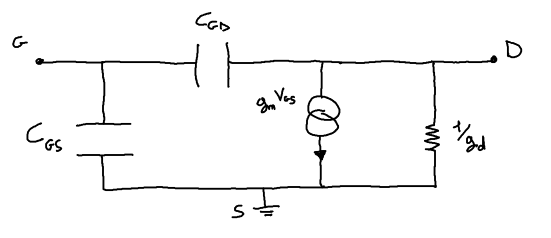
\includegraphics[width=0.5\textwidth]{smallsig.png}\\
\raggedright

We have only to link the values $C_g,C_d$ to the capacitance $C_{gd},C_{gs}$ we can do this considering a modulation of the drain/source with the other terminals grounded and probe what impedance we see; doing this procedure we get 
\begin{equation}
C_g=C_{gs}+C_{gd} \ \ \ \ \ \ C_d=C_{gd}
\end{equation}
In ohmic regime we get that $C_{gs}=C_{gd}=1/2WLC_{ox}$ while in saturation regime $C_d=C_{gd}\simeq 0$ ,$C_{gs}=2/3WLC_{ox}$ ; the phisical reason of this is that the drain loses control of the inversion charge only source provides electrons at the channel.\\

%------------------------------------------------------------------------%
\subsection{Frequency responce} 
The frequqncy responce is related to the transit time of the electrons in the channel so we can define it as 
\begin{equation}
\tau_t=\int_0^L \frac{dy}{v_d}
\end{equation}
recovering the definition used for the narrow base diod we get $\tau_t=Q_c/I_{ds}$ ;beacuse $Q_c$ isn't a linear function of $I_{ds}$ we can only use a small signal model so
\begin{equation}
\tau_t= -\frac{\partial Q_c}{\partial I_{ds}}= -\frac{\partial Q_c}{\partial V_{gs}}\frac{\partial V_{gs}}{\partial I_{ds}}=C_g \frac{1}{g_m}
\end{equation}
So in ohmic and saturation regimes we get
\begin{equation}
\tau_{ohm}=\frac{L^2}{\mu_nV_{ds}}\ \ \ \ \ \ \ \ \tau_{sat}=\frac{2}{3} \frac{L^2}{\mu_nV_{ds}}
\end{equation}
Smaller L we get smaller distance and grater electric field so grater velocity (over a smaller space).\\
Using the cutting frequency of the transistor we find that 
\begin{equation}
f_t=\frac{g_m}{2\pi (C_{gs}+C_{gd})}=\frac{1}{2\pi}\frac{g_m}{C_g}=\frac{1}{2\pi \tau_t}
\end{equation}

%------------------------------------------------------------------------%
\section{Body effect}
Until now we've always considered the bulk grounded now we consider the situation if we apply a $V_{bs}<0$ (with a positive voltage we will have the 2 junction forward biased). Total voltage under the channel is now $V_{gs}-V_{bs}$. We can restore the initial condition of substrate grounded if we add at all the other pins a voltage of $-V_{bs}$ like in figure\\

\centering
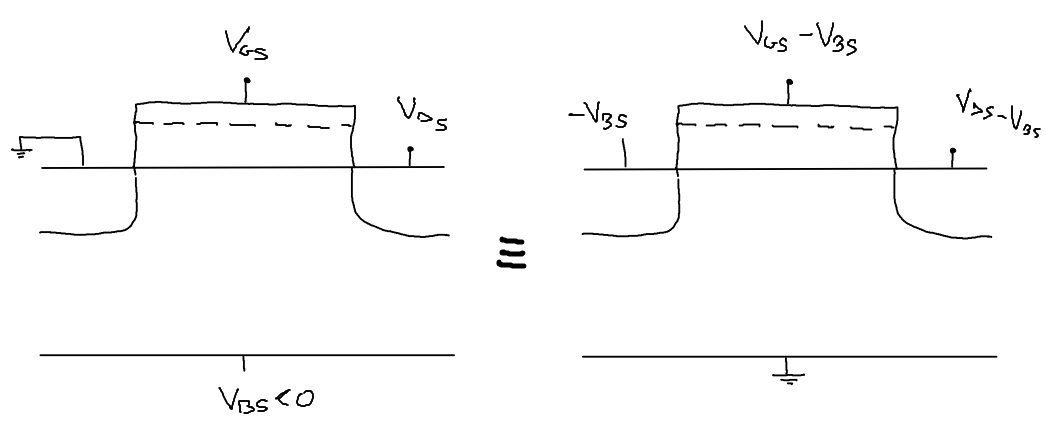
\includegraphics[width=0.5\textwidth]{body1.png}\\
\raggedright

In this case we get that $V_{gs}-V_{bs}-V_{fb}=V_s-Q_s/C_{ox}$ from this we get that che inversion charge is (under charge sheet approximation) 
\begin{equation}
Q_{inv}=Q_s-Q_{dep}=-C_{ox}(V_{gs}-V_{bs}-V_{fb}-V_s)+\sqrt{2\varepsilon_{si}qN_aV_s}
\end{equation}
In ohmic regime $V_s\simeq 2|\phi_b|-V_{bs}$ so we get a change of the band diagram where also at the source $E_{fn}$ is under $E_{fp}$ \\

\centering
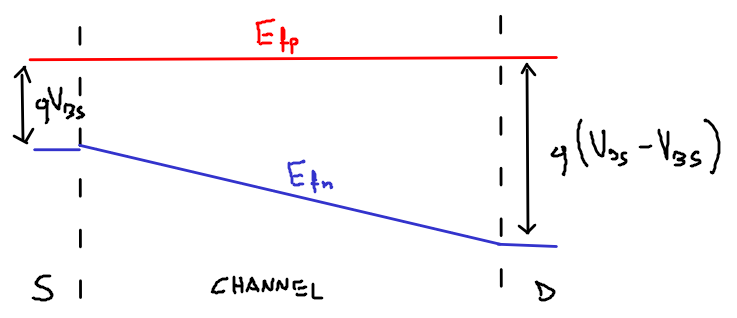
\includegraphics[width=0.35\textwidth]{body2.png}\\
\raggedright

making a little bit of calculation we get that in ohmic regime
\begin{equation}
Q_{inv}=-C_{ox}(V_{gs}-V_{fb}-2|\phi_b|-\frac{\sqrt{2\varepsilon_{si}qN_a(2|\phi_b|-V_{bs})}}{C_{ox}})=-C_{ox}(V_{gs}-V_t')
\end{equation}
$V_t'$ is the new threshold voltage of the system and we get $I_{ds}=\mu_nC_{ox}\frac{W}{L}(V_{gs}-V_t')V_{ds}$ this expression is equal to the one with the bulk grounded but with another $V_t$. For the other regimes we get the same resuslts of bulk grounded with $V_t'$ and for the parabolic regime m is modified.\\

\centering
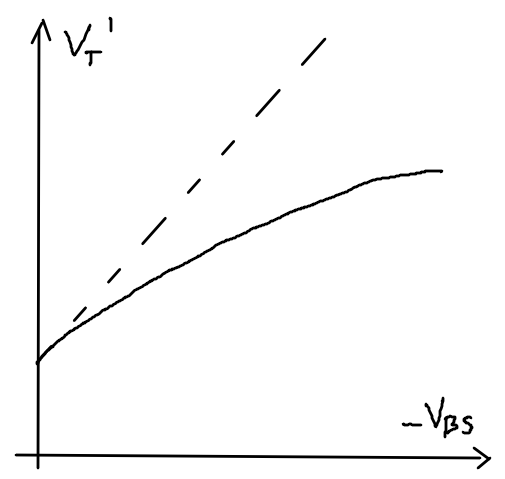
\includegraphics[width=0.2\textwidth]{body3.png}\\
\raggedright

For better undestand the behaviour of $V_t'(-V_{bs})$ we can study 
\begin{equation}
\frac{d V_t}{dV_{bs}}|_{V_{bs}=0}=[\frac{\sqrt{2\varepsilon_{si}qN_a}}{C_{ox}}\frac{1}{2}\frac{1}{\sqrt{2|\phi_b|-V_{bs}}}]|_{V_{bs}=0}=\frac{C_{dep}}{C_{ox}}=m-1
\end{equation}

%------------------------------------------------------------------------%
\section{Subtheshold regime}
%------------------------------------------------------------------------%

%------------------------------------------------------------------------%
\subsection{Current expression}

\centering
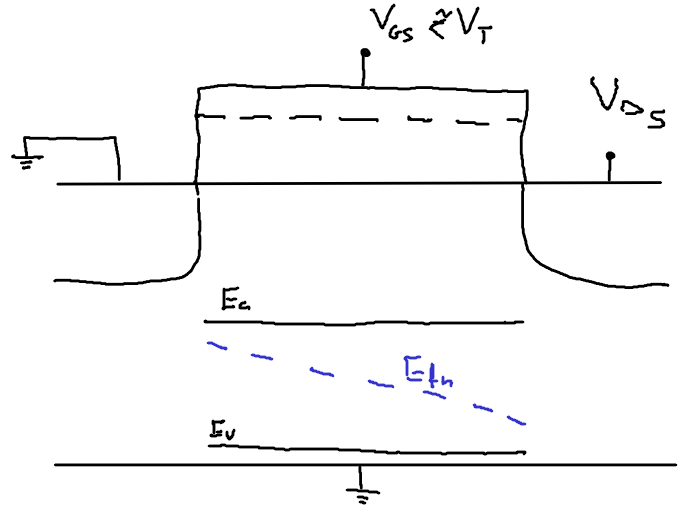
\includegraphics[width=0.35\textwidth]{subth.png}\\
\raggedright

In this regime $V_{gs} \lesssim V_t$ so we don't have strong inversion anywhere in the channel, the electron concentration is negligible for electrostatics that is dominated by the depletion charge. Bands are almost flat in the channel (also if electorn concentation change beacuse it's a neglibile contribution).\\
We get a diffusion current of electrons the drift flow is negligible. Solving the poisson equation we got that $Q_{inv}=-\sqrt{\frac{\varepsilon_{si}qN_a}{2V_s}}\frac{kT}{q}\frac{n_i^2}{N_a^2}e^{q(V_s-V)/kT}$ we can use this expression to derive the current in this regime so 
\begin{equation}
I_{ds}=-\mu_n \frac{W}{L}\int^{V_{ds}}_0-\sqrt{\frac{\varepsilon_{si}qN_a}{2V_s}}\frac{kT}{q}\frac{n_i^2}{N_a^2}e^{q(V_s-V)/kT}dV
\end{equation}
We can extract form the integral the square root and $V_s$ beacuse they are not function of y of V so 
\begin{equation}
I_{ds}=\mu_n \frac{W}{L}\sqrt{\frac{\varepsilon_{si}qN_a}{2V_s}}\frac{kT}{q}\frac{n_i^2}{N_a^2}e^{qV_s/kT}\int^{V_{ds}}_0e^{-qV/kT}dV
\end{equation}
Solving the integral we get the following expression
\begin{equation}
I_{ds}=\mu_n \frac{W}{L}\sqrt{\frac{\varepsilon_{si}qN_a}{2V_s}}\left(\frac{kT}{q}\right)^2\frac{n_i^2}{N_a^2}e^{qV_s/kT}\left(1-e^{-qV_{ds}/kT}\right)
\end{equation}
we want a dependance on $V_{gs}$ not on $V_s$.\\
As done for the MOS capacitor we use $V_{gs}-V_{fb}=V_s+\sqrt{2\varepsilon_{si}qN_aV_s}/C_{ox}$ we can assume that $V_s \lesssim 2|\phi_b|$ so we can make a Taylor expansion of $\sqrt{V_s}$ over $2|\phi_b|$ getting 
\begin{equation}
\sqrt{V_s}\simeq \sqrt{2|\phi_b|}+\frac{1}{2}\frac{V_{s}-2|\phi_b|}{\sqrt{2|\phi_b|}}
\end{equation}
(remember f(a)+f'(a)(x-a)). Replacing this expression in the previous formula we get 
\begin{equation}
V_{gs}=V_{fb}+V_s+\sqrt{2\varepsilon_{si}qN_a2|\phi_b|}/C_{ox}+\frac{1}{2}\frac{V_{s}-2|\phi_b|}{\sqrt{2|\phi_b|}}\sqrt{2\varepsilon_{si}qN_a}/C_{ox}
\end{equation}
adding and removing $2|\phi_b|$ we can write that expression as 
\begin{equation}
V_{gs}=V_t+(V_s-2|\phi_b|)m\ \ \ \ \ \ \ \rightarrow \ \ \ \ \ V_{s}=2|\phi_b|+\frac{V_{gs}-V_t}{m}
\end{equation}
The physical meaning of this can be explained considering a system like in fiure\\

\centering
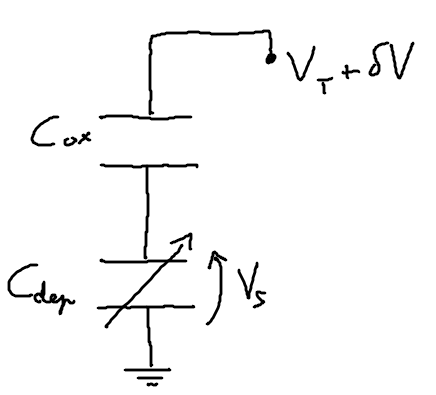
\includegraphics[width=0.2\textwidth]{subth2.png}\\
\raggedright

where we can say that $V_s=2|\phi_b|+\delta V \frac{C_{ox}}{C_{ox}+C_{dep}}=2|\phi_b|+\frac{\delta V}{m}$.\\
Turning back the the expression for the current we can write it in this way now
\begin{equation}
I_{ds}=\mu_nC_{ox}(m-1)\frac{W}{L}(\frac{kT}{q})^2 e^{q(V_{gs}-V_t)/mkT}\left(1-e^{-qV_{ds}/kT}\right)
\end{equation}
That is the expression for the current in the subtheshold regime. If $V_{ds}$ is more than a few kT the last exponential can be neglected.\\

\vspace{5mm}

The current density $J_n$ is a pure diffusion process so we can say that $J_n=qD_n \frac{dn}{dy}$ and so
\begin{equation}
I_{ds}=-W\int^{t_{inv}}_0qD_n \frac{dn}{dy}dx=WD_n \frac{d}{dy}\left(\int^{t_{inv}}_0 -qndx\right)=WD_n \frac{d}{dy}Q_{inv}
\end{equation}
This means that $Q_{inv}$ has to change linearly over y (stationary case without G-R so current constant over y) so that 
\begin{equation}
I_{ds}=-WD_n \frac{Q_{inv}(0)-Q_{inv}(L)}{L}
\end{equation}
where we remember that 
\begin{equation}
Q_{inv}(0)=\sqrt{\frac{\varepsilon_{Si}qN_a}{2V_s}}	\frac{kT}{q}\frac{n_i^2}{N_a^2}e^{q\frac{V_s}{kT}}
\end{equation}
\begin{equation}
Q_{inv}(L)=Q_{inv}(0)e^{q \frac{V_s-V_{ds}}{kT}}
\end{equation}
Since the change of charge is linear $E_{fn}$ must drop logaritmically.\\


%------------------------------------------------------------------------%
\subsection{Transcaracteristics}
%------------------------------------------------------------------------%

\begin{wrapfigure}{i}{0pt}
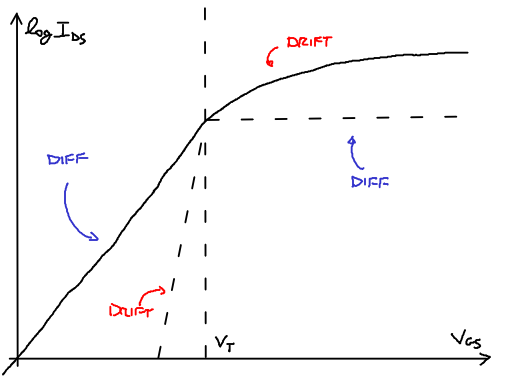
\includegraphics[width=0.35\textwidth]{tranclog.png}
\end{wrapfigure}

Let's plot now $I_{ds}(V_{gs})$ in a logaritmic plot. We obtain for the subtheshold regime a rect with a slope defined as sub-theshold slope or STS of 
\begin{equation}
STS=\left(\frac{\partial \log(I_{ds})}{\partial V_{gs}}\right)^{-1}=\frac{kT}{q}\ln(10)m
\end{equation} 
At room temperature STS=(60 mV/dec)m.\\ 
Form $V_t$ on the diffusion contribution to the current saturates and the drift becomes dominant.\\
If we move to low current we break the assumption of flat band condition $V_s$ becomes indipendent on $V_{gs}$ (near and below the FB condition) so our expression is no more valid and the current will saturate to a lower value.\\
At low current we have to take also in account the GR processes in the channel. We have a net generation process beacuse $E_{fn}<E_{fp}$ and also form the reversed bias junctions form drain-bulk. Generated electrons will assist the current flow. Tipically before breaking the assumption of flat-band the current saturate due to the G process.\\

\centering
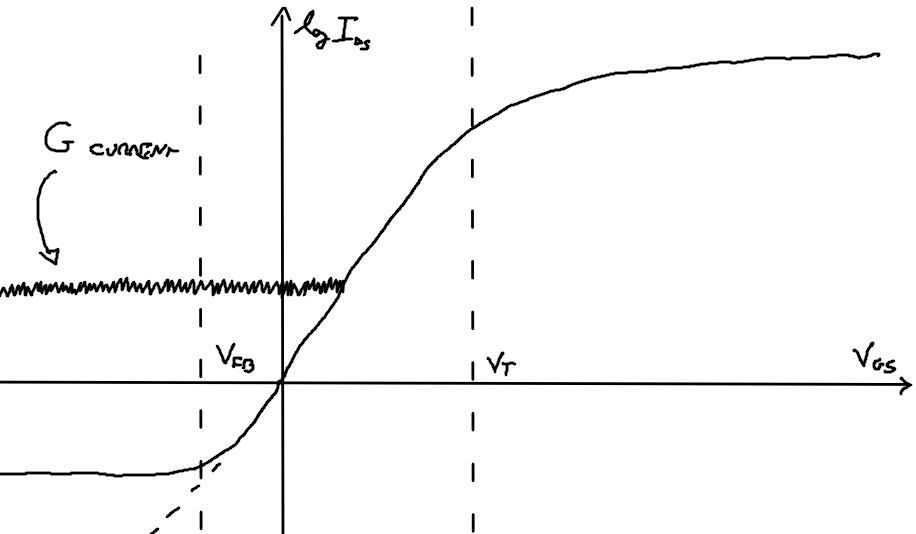
\includegraphics[width=0.4\textwidth]{noisefloor.png}\\
\raggedright

%------------------------------------------------------------------------%
\subsubsection{Improvment for MOS}
If we reduce $t_{ox}$ the gate will have better control of the substrate and better $STS=\frac{kT}{q}\ln(10)(1+(\varepsilon_{si}t_{ox})/(\varepsilon_{ox}W_d^{max}))$ and also lower $V_t\propto|Q_{dep}^{max}|/(\varepsilon_{si}/t_{ox})$.\\
It's also good to decrease $N_a$ to better deplete the substrate getting better STS and lower $V_t$


%------------------------------------------------------------------------%
\section{Temperature dependance}
%------------------------------------------------------------------------%
In sub-threshold regime the STS with high temperatures becomes higher and so we have a curve less steeper (rect more flat).\\


\centering
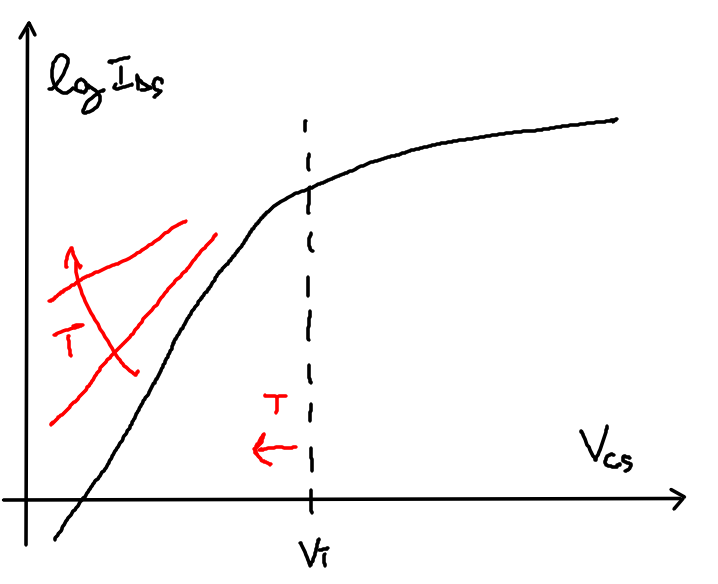
\includegraphics[width=0.35\textwidth]{tchange.png}\\
\raggedright

We have a change also of the $V_t$; $\phi_b$ change, with T also $E_f$ change ans so the flat band voltage and also $E_{f(m)}$ change depending on what metal we are using.\\


\centering
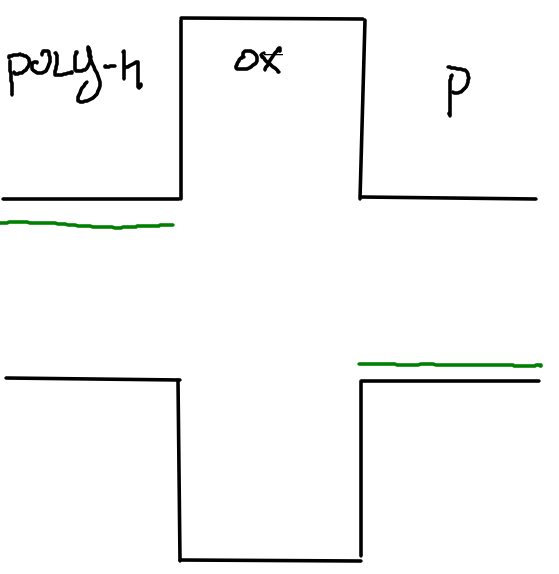
\includegraphics[width=0.15\textwidth]{1tchange.png}\\
\raggedright


Using a polysilicon gate as in figure we can say that $V_{fb}=-(\frac{E_{gap}}{2q}+|\phi_b|)$ so we can write 
\begin{equation}
V_t=-\frac{E_{gap}}{2q}+|\phi_b|+\frac{\sqrt{2\varepsilon_{Si}qN_a2|\phi_b|}}{C_{ox}}
\end{equation}
so we can study the derivative of this wrt T
\begin{equation}
\frac{dV_t}{dT}=-\frac{1}{2q}\frac{dE_{gap}}{dT}+\frac{d|\phi_b|}{dT}+\frac{\sqrt{2\varepsilon_{Si}qN_a2}}{C_{ox}}\frac{1}{2\sqrt{|\phi_b|}}\frac{d|\phi_b|}{dT}=-\frac{1}{2q}\frac{dE_{gap}}{dT}+\frac{d|\phi_b|}{dT}(2m-1)
\end{equation}
Inside $|\phi_b|=\frac{kT}{q}\ln(N_a/n_i)$ we have temperature dependances with T and $n_i$ so 
\begin{equation}
\frac{d|\phi_b|}{dT}=\frac{k}{q}\ln(N_a/n_i)-\frac{kT}{q}\frac{1}{n_i}\frac{dn_i}{dT}
\end{equation}
as last term we have to consider that $n_i=\sqrt{N_cN_v}e^{-E_{gap}/2kT}$ is strongly dependent on temperature so 
\begin{equation}
\frac{dn_i}{dT}=\frac{3}{2}aT^{1/2}e^{-E_{gap}/2kT}+aT^{3/2}e^{-E_{gap}/2kT}\left(\frac{-\frac{dE_{gap}}{dT}2kT+E_{gap}2k}{(2kT)^2}\right)
\end{equation}
Putting all this results in the first expression we get the final expression
\begin{equation}
\frac{dV}{dT}=-(2m-1)\frac{k}{q}\left(\ln(\frac{\sqrt{N_cN_v}}{N_a})+\frac{3}{2}\right) +\frac{m-1}{q}\frac{dE_{gap}}{dT}
\end{equation}
That is negative $\simeq -1mV/K$.\\
This phenomena have the effect to increase the offstate current.\\
With higher T also the mobility decrease and so the current.\\


%------------------------------------------------------------------------%
\section{Effects of non idealities}
%------------------------------------------------------------------------%

%------------------------------------------------------------------------%
\subsection{Parasitic resistance of $n^+$ regions}


\centering
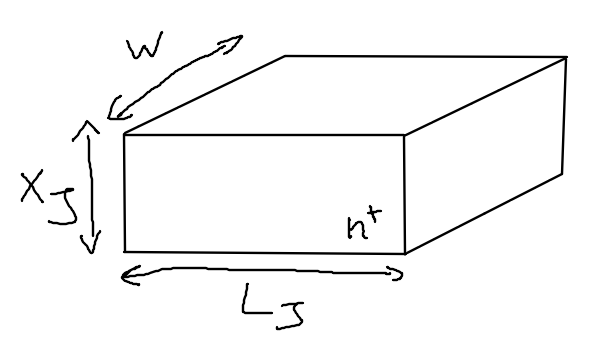
\includegraphics[width=0.35\textwidth]{parasR1.png}\\
\raggedright

Since $n^+$ regions are subjected to a flow of current they will show a resistance (that we suppose small since they are highly doped).\\
We computed the resistivity as $R=\rho_{sh}\frac{L}{W}$ putting some reasonable results we get a $\rho_{sh}=125 \Omega/sq$ that is reasonably higher than that of a metal so we have to consider it.\\


\centering
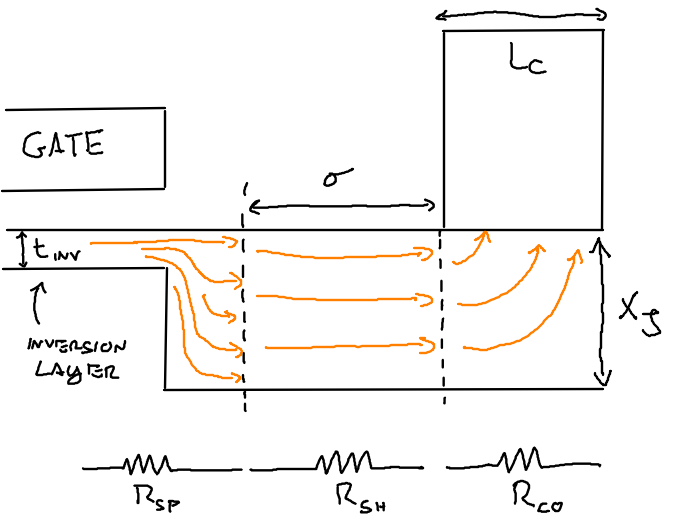
\includegraphics[width=0.45\textwidth]{parasR2.png}\\
\raggedright


We have other 2 contributions over $\rho_{sh}$ due to this parasitic resistances; vertical spreading of the electrons beacuse they are no more subjected by an electric field and the contact resistivity.\\
We can study this effects supposing an ideal case where we have a step-like increase in thikness from $t_{inv}$ to $X_j$ as in figure.\\
\vspace{5mm}
The contribution due to the vertical spread is 
\begin{equation}
R_{sp}=\frac{2\rho_{n^+}}{\pi W}\ln(0.75 \frac{X_j}{t_{inv}})
\end{equation}
\vspace{5mm}
The contribution due to the finite resistance is as we said 
\begin{equation}
R_{sh}=\rho_{sh}\frac{\sigma}{W}
\end{equation}
\vspace{5mm}
The third contribution is 
\begin{equation}
R_{co}=\frac{\sqrt{\rho_{sh}\rho_c}}{W}\coth(L_c\sqrt{\frac{\rho_{sh}}{\rho_c}})
\end{equation}
where $\rho_c=(\frac{\partial J}{\partial V})^{-1}$ is the contact resistivity.\\
This shows a different behaviour depending on $L_c$; with $L_c$ short the resistance incease in the "short contact" regime.\\
\vspace{5mm}
The average resistance is $R=R_{sp}+R_{sh}+R_{co}\simeq 302 \Omega\mu m/W$.\\
This can be modeled as resistance in series with source and drain that has the effects of reducing the actual $V_{ds}$; they have a relevant importance if the current is higher. If $V_{gs}$ is increased too much the channel resistance becomes too low and the current is setted by $R_s \ \ R_{d}$.\\
\vspace{5mm}
In scaling process $R_{ch}=\rho_{ch}\frac{W}{L}$ reducing L we arrive at $R_{ch}<<R_{s,d}$ at lower gate voltages this limiting the device.\\
In order to avoid this problems we deposit composit material like $TiSi_2$ over the contact; this has a small resistance and already act as a contact with silicon. This treatment is also applied to the gate to avoid parasitic resistance that will decrease f responce.\\

%------------------------------------------------------------------------%
\subsection{Parasitic capacitance}


\centering
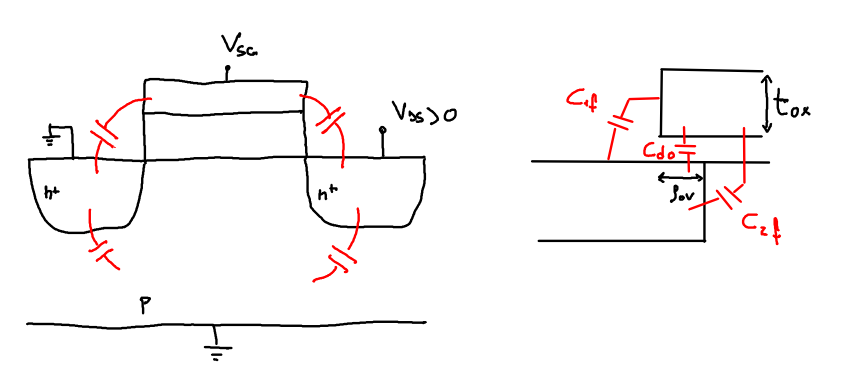
\includegraphics[width=0.5\textwidth]{parC.png}\\
\raggedright


We can identify $n^+-p$ junctions capacitance and gate coupling capacitnace.
The latter one can be divided in finge and direct overlapped capacitance that are
\begin{equation}
C_{1f}=\frac{2\varepsilon_{ox}W}{\pi}\ln(1+\frac{t_g}{t_{ox}})
\end{equation}
\begin{equation}
C_{2f}=\frac{2\varepsilon_{si}W}{\pi}\ln(1+\frac{X_j}{2t_{ox}})
\end{equation}
\begin{equation}
C_{do}=\frac{\varepsilon_{ox}}{t_{ox}}\rho_{ov}W
\end{equation}
that are in the order of fraction of fF ($C_{g}\simeq 1 fF$).

%------------------------------------------------------------------------%
\subsection{Leakage current}


\centering
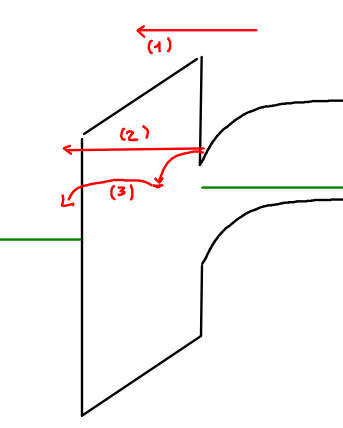
\includegraphics[width=0.25\textwidth]{leak1.png}\\
\raggedright


Considering the band diagram of a mos; electrons tend to move form substrate to the gate and they can reach this goal in three diffent methods. Thermionic transport is the first (1) which is difficult at room temperature due to the high barrier created by the oxide. The other 2 processes are quantum-mechanical tunneling indipendently (2) or with the help of a difect in the $SiO_2$ (3),or trap-assisted tunneling.\\
At RT with a low density of difect the most important contribution comes from the simple tunneling whose relevance grows as the oxide thikness is reduced.\\
Refering to the k space we are interested only in the right part of the parabola (electrons form Si to oxide) the current density is given by each electron ($\frac{q}{L^3}v_x(k_x)$) the barrier transparancy ($T(E_x)$) the probability of a state to be filled ($f(k_x,k_y,k_z)$) and the spin degeneracy (2) so we get 
\begin{equation}
J_{s-ox}=\sum_{k_x>0}2 \frac{q}{L^3}v_x(k_x)T(E_x)f(k_x,k_y,k_z)
\end{equation}
that becomes 
\begin{equation}
J_{s-ox}=\frac{1}{(\frac{2\pi}{L})^3}\int_{0}^{+\infty}\int_{-\infty}^{+\infty}\int_{-\infty}^{+\infty}\frac{q}{L^3}T(E_x)v_x(k_x)f(k_x,k_y,k_z)dk_xdk_ydk_z
\end{equation}
the integrals can be computed by considering $dk_{x,y,z}=\frac{m_{x,y,z}}{\hslash}dv_{x,y,z}$.\\
The difference wrt the metal-semiconductor junction is that here we have to use the Fermi-Dirac distribution for f beacuse we are intrested in states near $E_f$.\\
We can obtain that the current density as 
\begin{equation}
J=\frac{q\sqrt{m_ym_z}kT}{2\pi^2\hslash^3}\int^{+\infty}_0T(E_x)\ln(1+e^{-(E_x-E_f)/kT})dx
\end{equation}
where $T(E_x)$ can be computed using the WKB approximation.\\
In particular under Fouler-Nordheim tunneling 
\begin{equation}
J=AF_{ox}^2e^{-B/F_{ox}}
\end{equation}
Increasing the field in the oxide we enter in the direct tunneling regime being the boundary condition $\hat{F_{ox}}=\frac{q\xi_s}{t_{ox}}$. Typical values are arount J=1 A/$cm^2$.


\centering
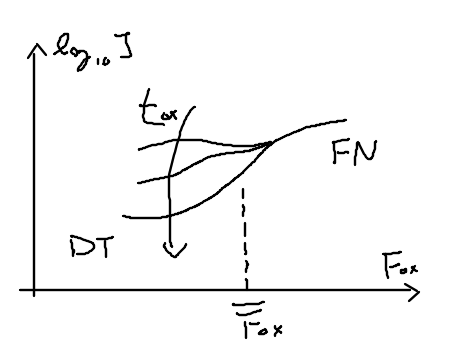
\includegraphics[width=0.35\textwidth]{fndt.png}\\
\raggedright


%------------------------------------------------------------------------%
\subsection{Charge in the oxide}

\centering
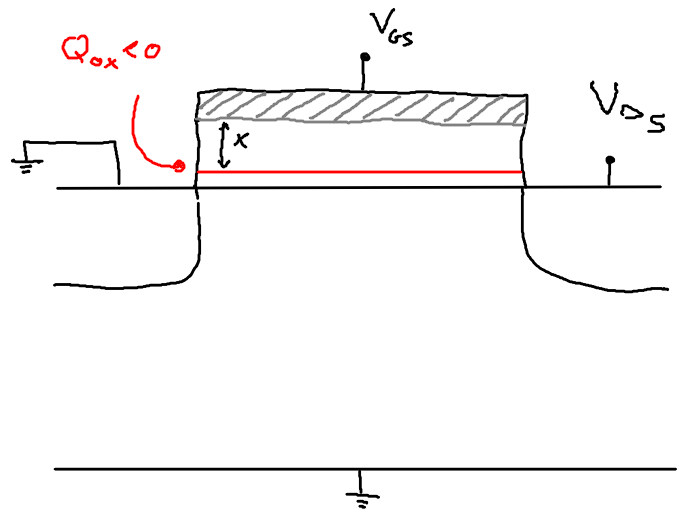
\includegraphics[width=0.35\textwidth]{qox.png}\\
\raggedright

We will consider a sheet of negative charge in the oxide at distance x from the gate. In MOS-capacitor we recover the ideal behaviour with the application of an extra voltage on the gate of 
\begin{equation}
\Delta V_g=-\frac{Q_{ox}}{C_{xg}}
\end{equation}
this consideration is also good for MOS-transistor. We have only a rigid shift of the transcaracteristic by an amount $\Delta V_{gs}$ that will be rightward if the charge is negative or lefward if positive.\\
This phenomena is used adding a strate of poly-silicon in the oxide called floating gate like in figure.\\
Depending at the charge given at a certain $\overline{V}$ we get different values of current. The charge in the floating gate is changed by quantum mechanical tunneling or other processes.\\

\centering
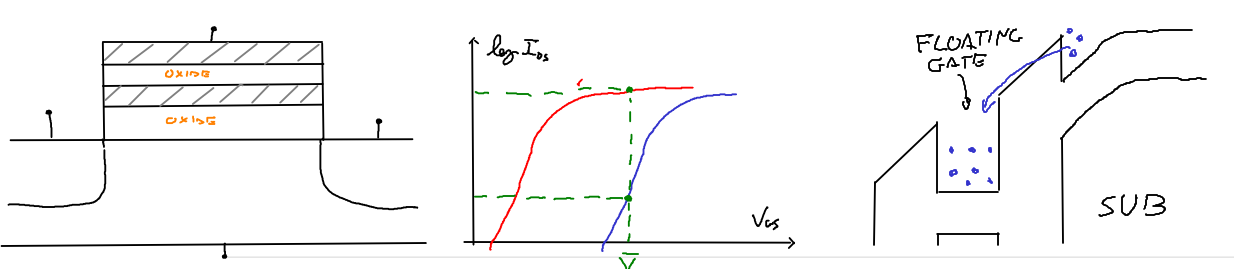
\includegraphics[width=0.9\textwidth]{flatinggate.png}\\
\raggedright


%------------------------------------------------------------------------%
\subsection{Interface states}
We get the same consideration of the MOS-capacitor.\\
Now the change of charge at the surface is modulating the slope of the sub-threshold slope. It's like having another capacitance in parallel with $C_{dep}$ so
\begin{equation}
STS=\frac{kT}{q}\ln(10)\left(1+\frac{C_{dep}+C_{i,s}}{C_{ox}}\right)
\end{equation}
We don't have a strech of the characteristic when $E_f=E_{i,s}$

\centering
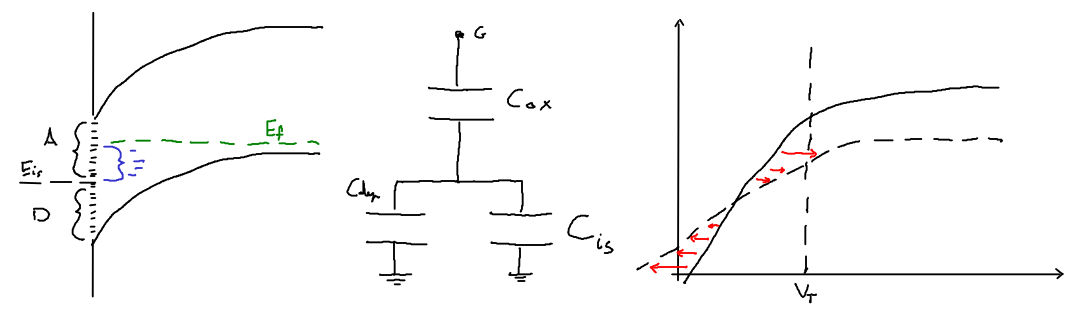
\includegraphics[width=0.7\textwidth]{interfacest.png}\\
\raggedright


%------------------------------------------------------------------------%
\section{Short channel devices}
%------------------------------------------------------------------------%

Reducing L we can increase the number of components per unit area and so decrease the costs per component and logic function. Furthermore
\begin{equation}
I_{ds}\propto \frac{W}{L} \ \ \ \ \ C\propto WL \ \ \ \ \rightarrow \ \ \ \ \ \frac{I_{ds}}{C}=\frac{dV}{dt}\propto \frac{1}{L^2}
\end{equation}
If we start reducing L leaving all the other parameters unchanged (like the oxide thikness or the doping concentrations) at the beginning the performance will increase but after a while they will become worst; this beacuse some secondary effects becomes dominants degrading the good performance of the transistor.

%------------------------------------------------------------------------%
\subsection{2D electrostatic in channel coming from $n^+$ regions}
In a long channel device with drain bias equal to 0 and $V_{gs} \lesssim V_t$ bands are flat in the channel and the electron concentration is negligible.\\

\centering
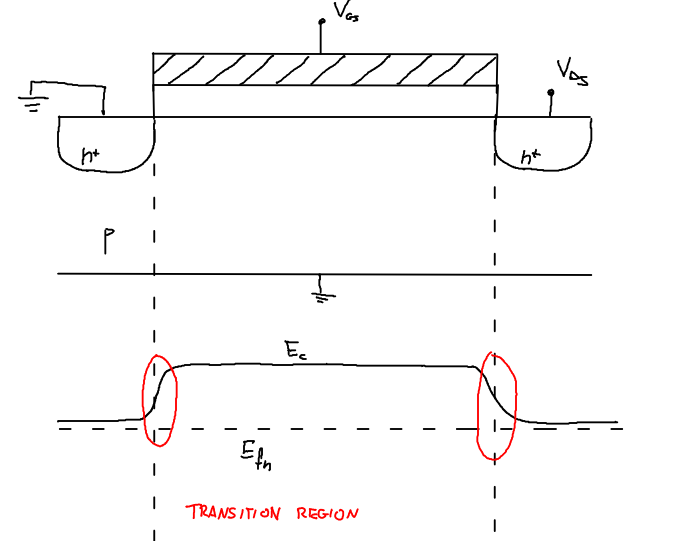
\includegraphics[width=0.5\textwidth]{longch.png}\\
\raggedright

In our analysis we've always neglected the presence of the source and drain regions (that untill now only setted the value of $E_{fn}$ at the boundary of the channel). We have 2 transition regions that we have neglected beacuse L is long and the thikness of this 2 region is negligible wrt L so they had a negligible impact.\\
If we reduce only L the electrostatics of the channel changes ; $E_c$ rises but not as much as before beacuse there is the influence of the drain transition region. We have everywhere an impact of the electrostatic of the source and drain regions we don't have a zone that can be controlled only by the gate.\\

\centering
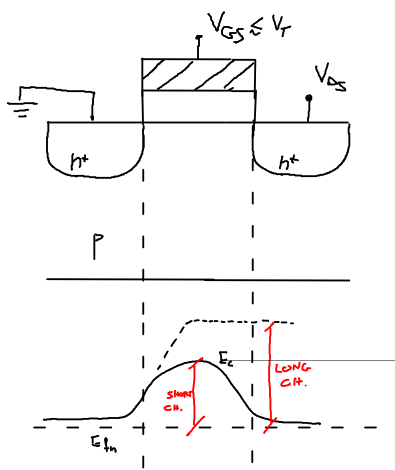
\includegraphics[width=0.35\textwidth]{shortch.png}\\
\raggedright

There are relevant electric field in y direction (gradient of $E_{fn}$) so an intrinsecally 2D electrostatic.\\
The distance $E_{fn}-E_c$ is narrower than before so we have more electrons that means we are reducing the $V_t$; this effect is called the short channel effect. Transistor with different L have different $V_t$. Variability on L will reflect on variability in $V_t$.\\

\centering
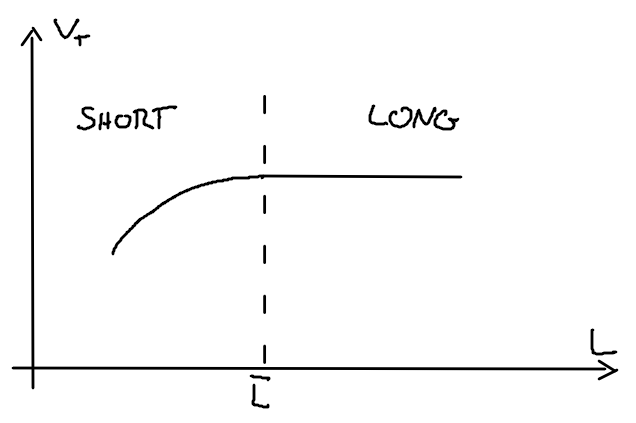
\includegraphics[width=0.35\textwidth]{shortcheff.png}\\
\raggedright

If now we increase $V_{ds}$ in short channel we change the electrostatic and the band banding moving $E_c^{max}$ to a lower value and near to the source as in figure.\\

\centering
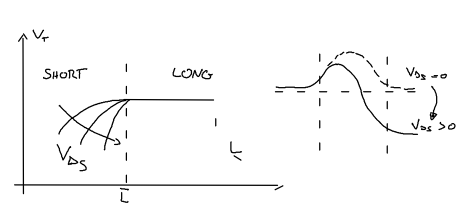
\includegraphics[width=0.5\textwidth]{dibl.png}\\
\raggedright

We are further reducing the $V_t$ of the transistor; this phenomena is called drain induced barrier lowering or DIBL. The effect is a decrease of the output resistance in the saturation regime.\\
In the transcharacteristic changing $V_{ds}$ we change $V_t$ increasing the on-state current exponentially and we have also a worstening of the STS that has a flatter dependance beacuse increasing $V_{ds}$ we decrease the barrier and $F_x$ becomes negligible wrt $F_y$.\\

\centering
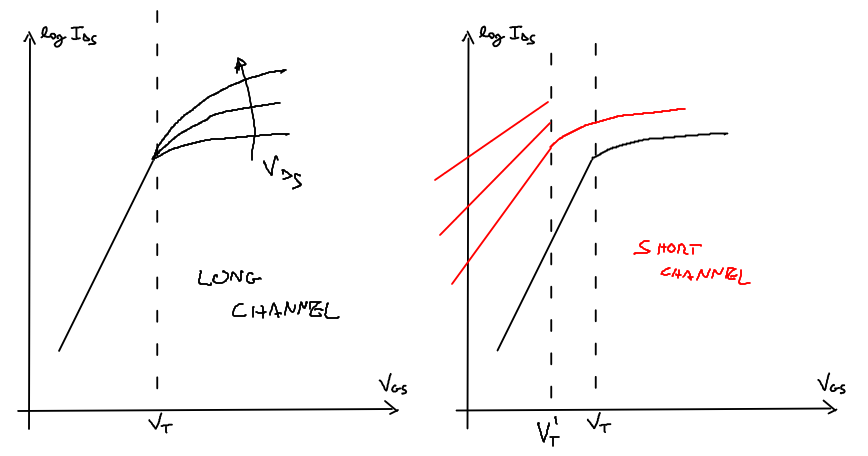
\includegraphics[width=0.5\textwidth]{shorttc.png}\\
\raggedright

This goes on until we have no barrier at all the gate is no more able to turn off the device; this condition is called punch-throught regime.\\
\vspace{5mm}
From the 2D Poisson equation we get that the difference of $V_t$ wrt a long channel device is 
\begin{equation}
\Delta V_t= \frac{24t_{ox}}{W_d^{max}}\left(\sqrt{\phi_b(\phi_b-V_{ds})}-0.4\cdot 2|\phi_b|\right)e^{-\pi L/2(W_d^{max}+3t_{ox})}
\end{equation} 
the importat term is the exponential.\\
To have a $\Delta V_t<100mV$ we need to have 
\begin{equation}
L>2(W_d^{max}+3t_{ox})
\end{equation}
if this condition is respected we have a long channel device if not a short channel. So we don't have an absolute value but a dependance con $t_{ox},N_a$ to separate long and short channel mosfets.\\
Reducing $t_{ox}$ we get a better control of the gate on the substate. With higher doping concentration the transitions regions are smaller but we get also a worst STS.\\

%------------------------------------------------------------------------%
\subsection{Velocity saturation}
Now let's forget about previous effects seen for short channel devices (we're making a sort of sovrapposition of effects).\\
Reducing L we are increasing F but at very high F we the relation between the electric field and the drift velocity isn't linear ; at fields of $10^4 V/cm$ the velocity of electrons saturates at a value of $10^7 cm/s$.\\

\centering
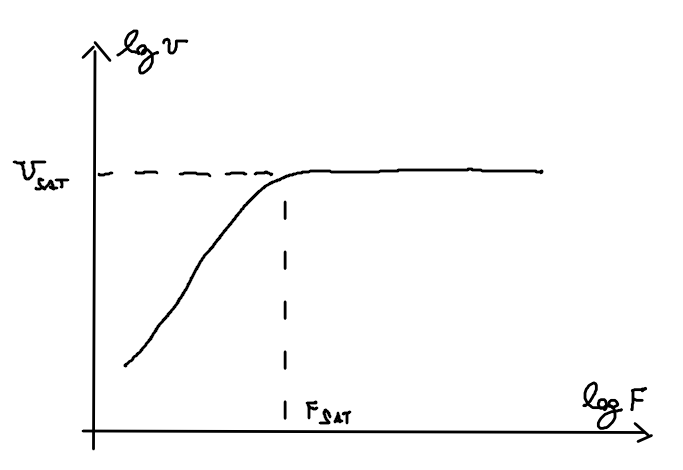
\includegraphics[width=0.3\textwidth]{satvel.png}\\
\raggedright

To express this dependence we can use the following formula 
\begin{equation}
v_d=\mu_{eff}\frac{F}{[1+\left(\frac{F}{F_{sat}}\right)^n]^{1/n}}
\end{equation}
where n is a coefficient equal to 1 for holes in a p-mos, 2 for electrons in n-mos.\\ 
The term $\mu_{eff}$ it's an effective mobility and depends on $F_x$; since the transport of electrons is very close to the surface there is a strong interaction with the interface Si-Oxide that causes surface-scattering events. The mobility in that region is much lower than that in the bulk and depends a lot on the vetical fields. We introduce also an effective vertical electric field as $F_{eff}=\frac{Q_{dep}+0.5Q_{inv}}{\varepsilon_{si}}$ that is related to the effective mobility as in the graph.\\

\centering
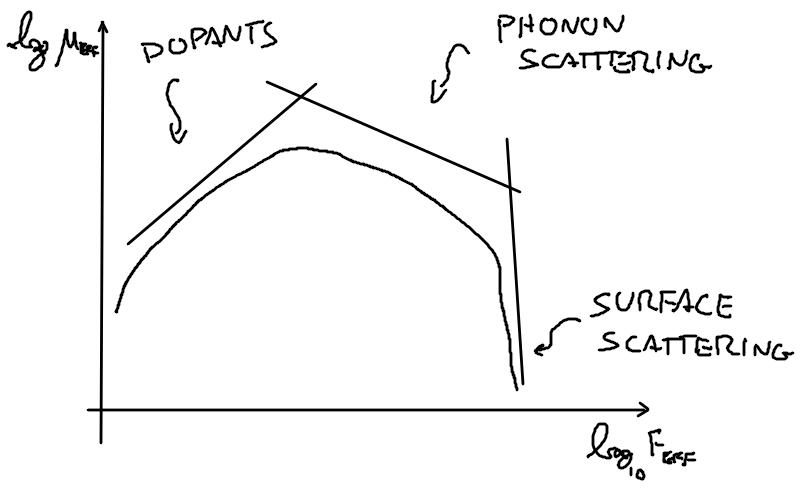
\includegraphics[width=0.35\textwidth]{muefff.png}\\
\raggedright

Now for the sake of semplicity we will consider n=1 in n-mos. We want to introduce velocity saturation expression in the current $I_{ds}=-\mu_nWQ_{inv}dV/dy$. Taking into account only the on-state regime we know that $V_s=2|\phi_b|+V$ and so that $dV_s/dy=dV/dy=-F_{y}$ in strong inversion regime so we arrive at 
\begin{equation}
\mu_n \frac{dV}{dy}=-\mu_nF_y=-v_d \ \ \ \ \ \rightarrow  \ \ \ \ \ \ \ I_{ds}=WQ_{inv}v_d
\end{equation}
So now we can introduce the velocity saturation equation in the expression (attention at the denominator we want a positive number so we take $|F|$)
\begin{equation}
I_{ds}=-WQ_{inv}\frac{\mu_{eff}\frac{dV}{dy}}{1+\frac{1}{F_{sat}}\frac{dV}{dy}}
\end{equation}
making some simple calculations we can write this equation like
\begin{equation}
I_{ds}=-[\mu_{eff}WQ_{inv}+\frac{I_{ds}}{F_{sat}}]\frac{dV}{dy}
\end{equation}
We can take dy to the first member and integrate from 0-L and form 0-$V_{ds}$; by assuming the quasi-1D model the only term that we really have to integrate is $Q_{inv}$ that we can write like $Q_{inv}=-C_{ox}(V_{gs}-V_t-mV)$ .\\
Solving the integral we get
\begin{equation}
I_{ds}=\frac{\mu_nC_{ox}\frac{W}{L}[(V_{gs}-V_t)V_{ds}-\frac{mV_{ds}^2}{2}]}{1+\frac{1}{F_{sat}}\frac{V_{ds}}{L}}
\end{equation}
We get the same expression of the ideal case but with the denominator that scales the current. With L long the denominator $\simeq 1$.\\
Decreasing L we get a decrease of the current wrt the long channel case.\\
This relation has got a maximum at 
\begin{equation}
V_{ds}^{sat}=\frac{2(V_{gs}-V_t)/m}{1+\sqrt{1+\frac{2(V_{gs}-V_t)}{F_{sat}mL}}}
\end{equation}
so we are reaching the saturation regime before than a long channel device and we get a higer slope of the rect after that point (Early's rect, this is also caused by the DIBLE). With a short L we get lower saturation voltage and saturation current.\\

\centering
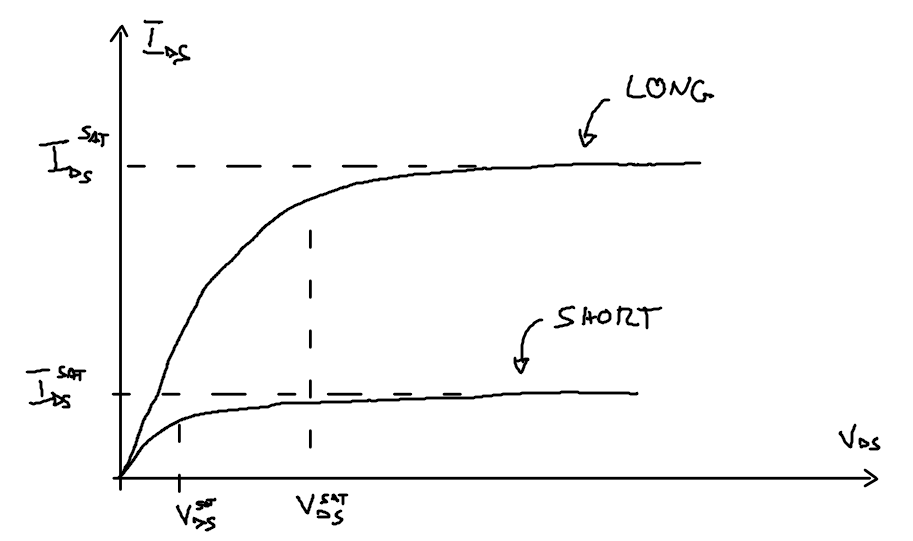
\includegraphics[width=0.35\textwidth]{ls.png}\\ %93up
\raggedright

If we consider the inversion charge at the drain interface at $V_{ds}^{sat}$ in a short channel device isn't zero we have still strong inversion. Before reaching pinch-off point at the drain we reach the saturation velocity; this 2 processes can lead our transistor in saturation region.\\
Ideally with shorter L we expect a steeper parabola in the transcaracteristic but we get considering the velocity saturation we get a high error. In an extreme case with $L\rightarrow 0$ $I_{ds}^{sat}\simeq WC_{ox}(V_{gs}-V_t)v_d^{sat}$ we get a linear dependance with $V_{gs}$ and we get a lower sensitivity of the current to gate changes.\\

\centering
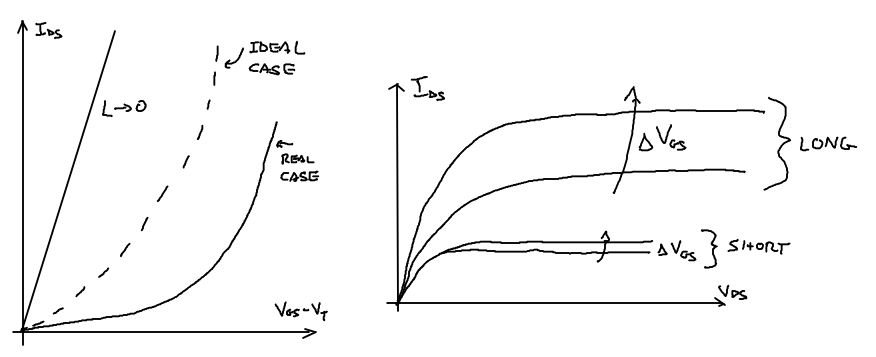
\includegraphics[width=0.75\textwidth]{shorta.png}\\
\raggedright

\subsubsection{Hot electrons}
The saturation velocity $v_{sat}$ is the maximum average velocity in a drift-diffusion framework and so with scattering events. We can avoid scattering events by using steeper band banding.\\

\centering
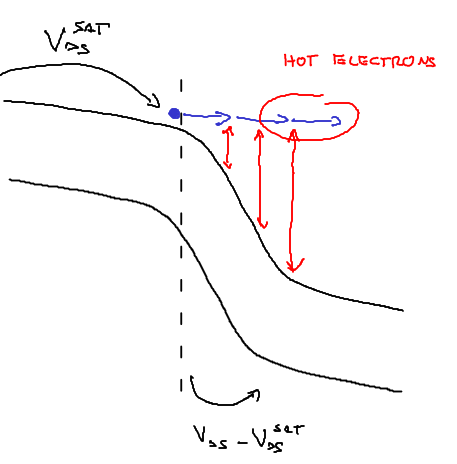
\includegraphics[width=0.35\textwidth]{hotelectrons.png}\\
\raggedright

Electrons that before scattering reaches a lot of kinetics energy (2-3eV) are called hot electrons. This electrons are so full of energy that can create impact ionization with atoms and so GR processes.\\
They can also inteact with silicon atoms at the surface breaking bonds and so creating some interface states. They are able to overcome the barrier of the oxide and reach the gate or remain trapped in the oxide ( they are used for floating gates charge processes).\\



%------------------------------------------------------------------------%
\section{Scaling rules}
%------------------------------------------------------------------------%
There are some sets of scaling rules that we can take as guideline to scale our devices.

%------------------------------------------------------------------------%
\subsection{Constant field (Dennard)}
Main idea is to avoid the 2D electrostatic regime keeping the ratio between the vertical and the horizontal fields constant $F_x/F_y=const.$\\
In order to do this we need to scale all vertical and horizontal dimensions of the same factor as the voltages.\\ 
For the doping concentrations we can say form the 2D Poisson equation in sub-threshold regime that 
\begin{equation}
\frac{\partial^2 \phi}{\partial x^2}+\frac{\partial^2 \phi}{\partial y^2}=\frac{qN_a}{\varepsilon_{si}}=-\frac{\partial F_x}{\partial x}-\frac{\partial F_y}{\partial y}
\end{equation}
and so scaling all dimension by a factor k we get that to have the same electrostatic conditions
\begin{equation}
\frac{qN_a'}{\varepsilon_{si}}=-\frac{\partial F_x}{\partial x/k}-\frac{\partial F_y}{\partial y/k}=-k\frac{\partial F_x}{\partial x}-k\frac{\partial F_y}{\partial y}
\end{equation}
from wch we get that $N_a'=kN_a$ so the doping concentrations must increase by a factor k.\\
So the rules for constant fields scaling are 
\begin{itemize}
  \item Dimensions (L,W,$t_{ox}$,$X_j$)     $\rightarrow \cdot 1/k$
  \item Voltages ($V_{gs},V_{ds},V_{bs}$)   $\rightarrow \cdot 1/k$
  \item Doping concentrations ($N_a,N_d$)   $\rightarrow \cdot k$
\end{itemize}

\subsubsection{Device parameters changes}
Electric field remains constant as the carriers velocity.\\
Capacitances scale as 1/k.\\
Taking into account the drain current in parabolic regime $I_{ds}=\mu_nC_{ox}\frac{W}{L}[(V_{gs}-V_t)V_{ds}-\frac{mV_{ds}^2}{2}]$ the current is scaled as 1/k but we have to consider the $V_t$ dependance. The threshold voltage has to be reduced by a factor k in accord with the second rule but we know that 
\begin{equation}
V_t=V_{fb}+2|\phi_b|+\frac{\sqrt{2\varepsilon_{si}qN_a2|\phi_b|}}{C_{ox}} \ \ \ \ \ \ \ \ \ \ C_{ox}\rightarrow \cdot k \ \ \ \ \ \ \ \ \ \ \ N_a \rightarrow \cdot k
\end{equation}
but $2|\phi_b|$ does not scale by a factor k we have a logaritmic dependance on the doping concentration ($2|\phi_b|=kT/q\ln(N_a/n_i)$). We are not free to modify as we want $V_t$ that is related with the energy gap and on $2|\phi_b|$. To overcome this we have to use non-costant doping concentrations.\\
The width of the depletion layer $W_d=\sqrt{\frac{2\varepsilon_{si}}{q}\frac{1}{N_a}2|\phi_b|}$ do not scale with k but less for it's dependance with $2|\phi_b|$. So scaling the device with this set of rules we are slowly moving to the short channel regime according to the formula 
\begin{equation}
L>2(W_d^{max}+3t_{ox})
\end{equation}
beacuse L scales as 1/k ,$t_{ox}$ scales as 1/k but due to the dependance of $W_{d}^{max}$ on $2|\phi_b|$ it scales less than 1/k.\\
Scaling also $V_t$ of k (supposing it possible) since the scaling process does not affect the STS we are exponentially increasing the off-power dissipation.\\
The transit time $\tau=L^2/(\mu_{eff}V_{ds})$ is scaled of 1/k so we are getting a better frequency responce.\\

\subsubsection{Circuit parameters changes}
\tab Delay of logic gates:\\
$CV/I_{ds}$ capacitances, current and voltage scale as 1/k so we get that the delay of logic gates decreases by a factor 1/k.\\
\tab Power dissipation:\\
$VI_{ds}$ both scale as 1/k so the power dissipation scales as $1/k^2$ we have less dissipated power per logic function.\\
\tab Density of power dissipation:\\
$\frac{VI_{ds}}{WL}$ the power dissipated per unit area remains constant (but we have more logic function in that area)\\
\tab Integration density:\\
1/WL number of device per unit area increase by a factor k\\

\vspace{5mm} %5mm vertical space

The negative aspects of this set of scaling rules are that we are slowly moving to short channel regime, we have higher off-power dissipation and we lose compatibility to one thecnology to the other scaling the voltages.


\subsection{Generalized scaling rules (Baccarjni)}
We accept an increase of F in order to move away from the 2D electrostatic regime (moving near to the velocity saturation regime).\\
\vspace{5mm}
With the same path of before we define the 3 rules of this set 
\begin{itemize}
  \item Dimensions (L,W,$t_{ox}$,$X_j$)     $\rightarrow \cdot 1/k$
  \item Voltages ($V_{gs},V_{ds},V_{bs}$)   $\rightarrow \cdot \alpha/k$
  \item Doping concentrations ($N_a,N_d$)   $\rightarrow \cdot \alpha k$
\end{itemize}
with $1<\alpha<k$ 

\subsubsection{Parameters change}
\tab Carrier velocity:\\
In the case of linear or low field regime $\cdot \alpha$ , in velocity saturation $\cdot 1$.\\
\tab Current:\\
In low field $\cdot \alpha^2/k$ , in velocity saturation $\cdot \alpha/k$.\\
\tab Capacitances:\\
The electric field is not involved so we get 1/k for every regime.\\
\tab Delay of logic gates:\\
In low field $\cdot 1/k$, in saturation $\cdot 1/k$.\\
\tab Power dissipation:\\
In low field $\cdot \alpha^3/k$, in saturation $\cdot \alpha^2/k$.\\
\tab Densisty of power dissipation:\\
In low field $\cdot \alpha^3/k^2$, in saturation $\cdot \alpha^2/k^2$ (we get problems form heat dissipation).\\

\vspace{5mm}

Increasing the doping concentration of more than k we get that $W_d^{max}$ decreases more so we don't reach short channel regime.\\
With $\alpha=k$ we keep the same voltages and so compatibility with the older processes.\\

\vspace{5mm}

Increasing F we are increasing hot electrons that can tunnel throught the gate that is becoming thinner so we get an exponential increase of the gate current with this process. In order to avoid this we use high-k material instead of $Si0_2$ increasing the thikness of the oxide but preserving the same capacitance so 
\begin{equation}
t_{ox}^{hk}=\frac{\varepsilon_{hk}}{\varepsilon_{ox}}t_{ox}
\end{equation}
However high-k materials are not so good in terms of charge inside the oxide, spurios states and interface states wrt $SiO_2$.\\ 

%------------------------------------------------------------------------%
\section{Constraint on electrical parameters}
%------------------------------------------------------------------------%

We know the formula for the STS that can be written as
\begin{equation}
STS=60 \frac{mV}{dec} \cdot m =60 \frac{mV}{dec} \cdot (1+\frac{C_{dep}}{C_{ox}})
\end{equation}
We want a low STS and so an $m\simeq 1$. Taking as upper limit $STS<85 \frac{mV}{dec}$ we get $m<1.4$ data from which we can elaborate the folloing formula 
\begin{equation}
m=1+\frac{C_{dep}}{C_{ox}}=1+\frac{\varepsilon_{Si}t_{ox}}{\varepsilon_{ox}W_d^{max}}\ \ \ \ \rightarrow \ \ \ \ \ t_{ox}<0.13W_d^{max}
\end{equation} 
We started from an electrical constraint to arrive to a phisical parameter.\\
\vspace{5mm}
Refrering to a long channel behaviour we can refer to the condition of $\Delta V_t^{short \ channel \ effect}=[...]e^{-\frac{\pi L}{2(W_{d}^{max}+3t_{ox})}}<100mV$ from this we get the well known equation $L>2(W_d^{max}+3t_{ox})$ that we can write to hilight the oxide thickness as 
\begin{equation}
t_{ox}<\frac{L}{6}-\frac{W_{d}^{max}}{3}
\end{equation}
\vspace{5mm}

Another constranint is the maximum electric field in the oxide so $\frac{V_{dd}}{t_{ox}}<F_{ox}^{max}$ and so 
\begin{equation}
t_{ox}<\frac{V_{dd}}{F_{ox}^{max}}
\end{equation}
\vspace{5mm}

We can study this 3 constraint on $t_{ox}$ in a graph $t_{ox}-W_d^{max}$\\

\centering
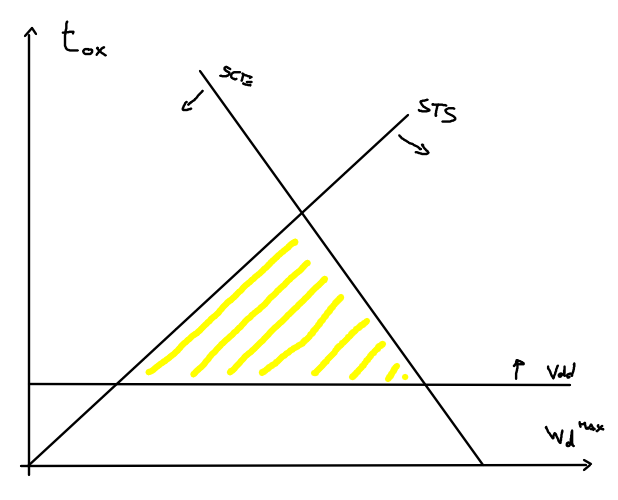
\includegraphics[width=0.35\textwidth]{trianglemos.png}\\
\raggedright

To satisfy the 3 requirements we have to stay in the triangle area and so we have a minimum and a maximum value for $t_{ox}$. In particular $t_{ox}^{max}\simeq \frac{L}{20}$; scaling L we have also to scale the oxide thickness increasing the leakage current through the gate.\\

\vspace{5mm}
Of course in the graph $t_{ox}^{max}>t_{ox}^{min}$ that means $V_{dd}<\frac{LF_{ox}^{max}}{20}$ but reducing the supply voltage we have also to reduce $V_t$ and doing so we increase the off-state current and power dissipation
From a requirement on off-power dissipation we can get the $I_{off}=I_{ds}^{V_{ds}=V_{dd} \ V_{gs}=0}$ and from sub-th current get the $V_t$ we want. We have to take the worst case so the one at high temperature and then come back to the RT. Olso we can't increase too much $V_t$ or the on-state current will be too low. Typical requirement is to have $V_t \le \frac{V_{dd}}{4}$\\

These constraint are why we came to "strange" structure like the finfet in figue \\

\centering
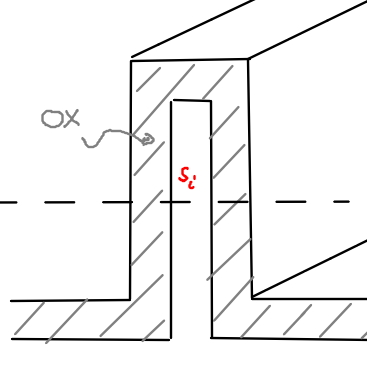
\includegraphics[width=0.35\textwidth]{finfet.png}\\
\raggedright

where we have a 3D channel controlled in a more strong way beacuse the gate wraps around the substrate over 2 dimensions having so a better STS and a volume inversion charge.
If we look at the band diagram in the crossection with $t_{si}$ large and small we can say that shorter the silicon thickness is better control of the substrate we have.\\

\centering
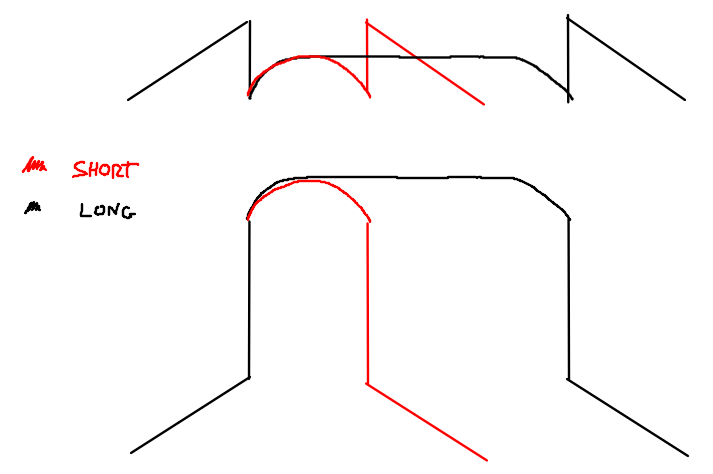
\includegraphics[width=0.35\textwidth]{finfetbd.png}\\
\raggedright

\section{Moore's Law and problems in the "too small"}
Moore's law :number of components per chip doubles every 2 years and so beacuse the area remains constant we get an integration density reduction of a factor $\sqrt{2}$ so we get 
\begin{equation}
45nm \rightarrow 32nm \rightarrow 22nm \rightarrow 14nm \rightarrow 10nm
\end{equation}

\vspace{5mm}
With so small spaces we have problems of statistical variability due to the intrinsic discrete nature of atoms; dopants are point charge not concentrations.\\

\centering
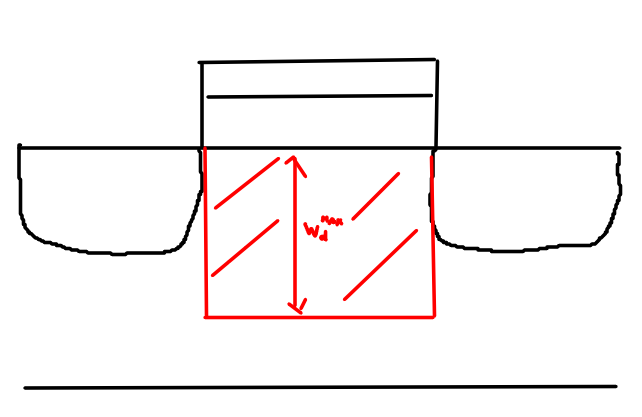
\includegraphics[width=0.15\textwidth]{mosrand.png}\\
\raggedright

In the area under the gate of a mos we have a certain nuber of dopants that can be calculated as $M=N_aWLW_d^{max}$ that for a 10nm thecnology are of a few thousand so variation of this nummber are very important and effective on the device behaviour.\\
Also with so few M it's relevant the position of them; we can have regions where the local $V_t$ is higher causing a non uniform inversion layer ad so a percolative substrate conduction.\\ 


\centering
\includegraphics[width=0.35\textwidth]{percolative.png}\\
\raggedright

